
\documentclass[journal]{IEEEtran}
\IEEEoverridecommandlockouts
\usepackage{cite}
\usepackage{amsmath,amssymb,amsfonts}
\usepackage{graphicx}
\usepackage{textcomp}
\usepackage{xcolor}
\usepackage{tikz}
\usepackage{pgfplots}
\usepackage{algorithm}
\usepackage{algpseudocode}
\usepackage{hyperref}
\usepackage{booktabs}
\usepackage{amsthm}
\usepackage{fontawesome5}
\pgfplotsset{compat=1.18}
\usetikzlibrary{positioning,arrows.meta,shapes.geometric,fit,backgrounds,calc}
\definecolor{ieeeblue}{RGB}{0, 102, 204}
\definecolor{ieeeorange}{RGB}{255, 128, 0}
\definecolor{seal}{RGB}{0,140,90}
\definecolor{glide}{RGB}{200,120,0}
\definecolor{tli}{RGB}{80,80,80}
\definecolor{teachbg}{RGB}{225,244,232}
\definecolor{querybg}{RGB}{240,231,246}
\definecolor{testbg}{RGB}{250,232,230}


% Visible placeholder for results/numbers still to be filled from experiments.
\newcommand{\todo}[1]{\textcolor{red}{\textbf{[TODO: #1]}}}
% Planned experiment/baseline not yet run (see TODO.md) -- blue to distinguish
% "experiment to run" from "number to fill in" (red).
\newcommand{\todoexp}[1]{\textcolor{blue}{\textbf{[PLANNED: #1]}}}

\theoremstyle{definition}
\newtheorem{definition}{Definition}
\newtheorem{assumption}{Assumption}
\theoremstyle{plain}
\newtheorem{proposition}{Proposition}
\theoremstyle{remark}
\newtheorem{remark}{Remark}

\begin{document}
\title{SEAL: Safe, Efficient Active Learning for\\ Task-Level Recovery in Long-Horizon Manipulation}

\author{Anonymous Authors% <-this % stops a space
}

\maketitle

%%%%%%%%%%%%%%%%%%%%%%%%%%%%%%%%%%%%%%%%%%%%%%%%%%%%%%%%%%%%%%%%%%%%%%%%%%%%%%%%
\begin{abstract}
Robust long-horizon manipulation requires a robot not only to execute a sequence of skills but to react at the \emph{task} level when real-world perturbations invalidate the nominal plan. A common formalism casts this as a hybrid automaton whose discrete modes (e.g., \textit{pick}, \textit{transport}, \textit{place}) select the active skill; the reactivity of the system then hinges on a \emph{localization function} that grounds the continuous state to the correct mode at runtime. Prior work either hand-engineers this grounding from temporal-logic specifications or learns it through self-supervised perturbation-and-reset rollouts that require unsafe failure data and an outcome oracle. We propose SEAL, an active-learning framework that instead learns the localization function directly from a handful of \emph{safe}, human-segmented demonstrations. SEAL (i) uses a large language model as a zero-shot semantic prior, verified by an information-theoretic observability check, to construct a minimal, spatially invariant feature space in which modes are instantaneously separable; (ii) trains a Gaussian Process Classifier whose epistemic uncertainty actively directs expert queries to under-determined regions of the state space; and (iii) exploits calibrated confidence at runtime to decouple switching latency from false-positive rate. Because the primitives are goal-directed dynamical systems, goal reachability holds by construction, and the learned classifier serves as a data-driven invariance monitor for detecting task-level failures. Across five simulated and real-world contact-rich tasks and a 10-participant user study, SEAL matches expert-tuned automata and self-supervised baselines while eliminating simulated resets, self-supervised rollouts, and dangerous failure data.
\end{abstract}

\begin{IEEEkeywords}
Learning from Demonstration, Hybrid Control, Task-Level Failure Recovery, Active Learning, Semantic State Estimation.
\end{IEEEkeywords}

%%%%%%%%%%%%%%%%%%%%%%%%%%%%%%%%%%%%%%%%%%%%%%%%%%%%%%%%%%%%%%%%%%%%%%%%%%%%%%%%

\begin{figure}[t!]
\centering
% New positioning figure: the task automaton is SHARED; only how the localization
% function L is obtained differs across TLI (hand-designed), GLiDE (learned via
% perturb+reset+oracle), and SEAL (learned from safe segmented demos).
\resizebox{\columnwidth}{!}{%
\begin{tikzpicture}[>=Latex, font=\small,
  mode/.style={circle, draw, thick, minimum size=7.5mm, inner sep=0pt},
]
% ---------- Top: the shared, designed automaton ----------
\node[mode] (a) {$a$};
\node[mode, right=12mm of a] (b) {$b$};
\node[mode, right=12mm of b] (c) {$c$};
\node[mode, right=12mm of c, double, double distance=1pt] (d) {$d$};
\node[above=0pt of a, font=\scriptsize] {Scoop};
\node[above=0pt of b, font=\scriptsize] {Transport};
\node[above=0pt of c, font=\scriptsize] {Deposit};
\node[above=0pt of d, font=\scriptsize] {Done};
\draw[->,thick] (a) -- (b);
\draw[->,thick] (b) -- (c);
\draw[->,thick] (c) -- (d);
\draw[->, thick, red] (b) to[bend left=48] node[below=0.5pt, midway, font=\tiny, red] {recovery} (a);
\begin{scope}[on background layer]
  \node[draw, dashed, rounded corners, inner xsep=4.5mm, inner ysep=6mm, fit=(a)(b)(c)(d)] (auto) {};
\end{scope}
\node[anchor=west, font=\bfseries\small] at ([yshift=1mm]auto.north west)
  {Designed task automaton \normalfont(shared by all three methods)};
\node[font=\scriptsize\itshape, below=0.5mm of auto.south]
  {reactivity $=$ localizing the state onto the correct mode: where is the guard?};

% ---------- Bottom: the SAME guard, obtained three ways ----------
% Panel geometry: width 3.5, height 2.7. True guard: load falls as tilt grows.
% Macro-ish: draw each panel in a shifted scope.
%
% ---- Panel 1: TLI (hand-placed thresholds, no data) ----
\begin{scope}[shift={(-1.35,-4.6)}]
  \draw[->] (0,0) -- (3.5,0) node[below left, font=\tiny] {tilt $\theta$};
  \draw[->] (0,0) -- (0,2.7) node[rotate=90, anchor=south east, font=\tiny] {load $F$};
  % true boundary (unknown to the designer)
  \draw[gray!70, thick, dashed]
    (0.25,2.15) .. controls (1.4,1.95) and (2.1,1.15) .. (3.2,0.55);
  \node[gray!70, font=\tiny, anchor=west] at (0.30,2.38) {true guard};
  % hand-placed axis-aligned thresholds
  \draw[tli, very thick] (1.6,0) -- (1.6,1.0) -- (3.3,1.0);
  \node[tli, font=\tiny, anchor=west] at (1.62,0.32) {$\theta\!>\!20^{\circ}$};
  \node[tli, font=\tiny, anchor=south west] at (2.35,1.02) {$F\!<\!0.5$N};
  % mismatch region
  \begin{scope}[on background layer]
    \fill[red!14] (1.6,1.0) -- (1.6,1.83) .. controls (2.0,1.5) and (2.4,1.2)
      .. (2.75,1.0) -- cycle;
  \end{scope}
  \node[red!70, font=\tiny, anchor=west] at (2.15,1.95) {mismatch:};
  \node[red!70, font=\tiny, anchor=west] at (2.15,1.70) {missed failures};
  % region labels: above the guard rice is retained, below it is lost
  \node[gray, font=\tiny\itshape, anchor=west] at (2.30,2.45) {$R_{\text{transport}}$: rice on};
  \node[gray, font=\tiny\itshape] at (0.85,0.40) {rice lost $\to$ Scoop};
  \node[font=\scriptsize\bfseries, tli, anchor=north] at (1.75,-0.42) {\faDraftingCompass~TLI: hand-placed};
  \node[font=\tiny, tli, anchor=north] at (1.75,-0.82) {no data consulted};
\end{scope}
%
% ---- Panel 2: GLiDE (fit to induced failures) ----
\begin{scope}[shift={(3.05,-4.6)}]
  \draw[->] (0,0) -- (3.5,0) node[below left, font=\tiny] {tilt $\theta$};
  \draw[->] (0,0) -- (0,2.7);
  % failure cloud (below/right of true boundary)
  \foreach \p in {(1.9,0.6),(2.3,0.85),(2.7,0.5),(2.5,1.0),(3.0,0.75),(2.1,0.35),
                  (2.85,0.32),(1.75,0.95),(2.45,0.6),(3.1,1.0),(2.05,1.12),(2.65,1.28)}
    \node[red!75, font=\tiny] at \p {$\times$};
  % success cloud (above/left)
  \foreach \p in {(0.5,1.7),(0.9,2.1),(1.3,1.75),(0.6,2.35),(1.6,1.6),(1.05,1.45),
                  (1.5,2.2),(0.35,1.35),(1.85,1.75),(0.85,1.75)}
    \fill[glide] \p circle (1.3pt);
  % fitted boundary hugs the truth
  \draw[glide, very thick]
    (0.25,2.15) .. controls (1.4,1.95) and (2.1,1.15) .. (3.2,0.55);
  % region labels + oracle legend
  \node[gray, font=\tiny\itshape, anchor=west] at (2.30,2.45) {rice on};
  \node[gray, font=\tiny\itshape] at (0.85,0.40) {rice lost};
  \node[glide, font=\tiny, anchor=west] at (0.15,0.15)
    {$\bullet$ valid\ \ \textcolor{red!75}{$\times$} invalid transition (oracle)};
  \node[font=\scriptsize\bfseries, glide, anchor=north] at (1.75,-0.42) {\faExclamationTriangle~GLiDE: fit to failure};
  \node[font=\tiny, glide, anchor=north] at (1.75,-0.82) {$1000$s of spills \faRedo\ resets + oracle};
\end{scope}
%
% ---- Panel 3: SEAL (fit to success only) ----
\begin{scope}[shift={(7.45,-4.6)}]
  \draw[->] (0,0) -- (3.5,0) node[below left, font=\tiny] {tilt $\theta$};
  \draw[->] (0,0) -- (0,2.7);
  % a few safe demonstration trajectories (stay on the safe side of the guard)
  \draw[seal!70, thick] (0.35,2.45) .. controls (1.0,2.5) and (1.5,2.15) .. (1.9,1.70);
  \draw[seal!70, thick] (0.5,2.25) .. controls (1.2,2.30) and (1.7,1.85) .. (2.2,1.45);
  \draw[seal!70, thick] (0.6,2.60) .. controls (1.5,2.55) and (2.0,1.85) .. (2.5,1.35);
  % query points proposed by the GPC at its most uncertain guard states
  \foreach \p in {(2.9,0.82),(2.55,1.08),(3.05,0.74)}{
    \fill[seal] \p circle (1.5pt);
    \draw[seal] \p circle (3.0pt);
  }
  \node[seal, font=\tiny, anchor=south west] at (2.55,1.55) {queries};
  % newly requested SAFE demos passing through the queried states (dashed)
  \draw[seal!70, thick, dashed] (2.05,1.65) .. controls (2.35,1.30) .. (2.55,1.08)
    .. controls (2.75,0.90) .. (3.05,0.74);
  \draw[seal!70, thick, dashed] (2.45,1.45) .. controls (2.70,1.10) .. (2.9,0.82)
    .. controls (3.00,0.73) .. (3.12,0.66);
  % region labels
  \node[gray, font=\tiny\itshape, anchor=east] at (3.35,2.20) {rice on};
  \node[gray, font=\tiny\itshape] at (0.85,0.40) {rice lost};
  % fitted boundary hugs the truth
  \draw[seal, very thick]
    (0.25,2.15) .. controls (1.4,1.95) and (2.1,1.15) .. (3.2,0.55);
  \node[font=\scriptsize\bfseries, seal, anchor=north] at (1.75,-0.42) {\faIcon{shield-alt}~SEAL: fit to success};
  \node[font=\tiny, seal, anchor=north] at (1.75,-0.82) {few safe demos + targeted queries};
\end{scope}
%
% connective tissue: all three feed the same L
\node[font=\scriptsize\itshape] at (4.8,-6.9)
  {three ways to obtain the same object: the localization function $L:\ \mathcal{X}_{\min}\!\to\!\mathcal{M}$};
\end{tikzpicture}%
}
\caption{\textbf{One automaton, one guard, three ways to find it.} \emph{Top:} all methods share the same designed automaton for scooping; reactivity reduces to knowing where the \emph{guard} lies in feature space (spoon tilt $\theta$ vs.\ load $F$). In each bottom panel the dark curve is that guard, separating \textit{Transport} still valid (rice on) from physically failed (rice lost $\to$ re-localize to \textit{Scoop}). TLI~\cite{wang2022temporal} places it by hand: where the analytic rule and the true boundary disagree (shaded), failures go undetected and no data corrects it. GLiDE~\cite{wang2024grounding} fits it to perturbed rollouts labeled by an outcome oracle---accurate, but at the cost of thousands of induced failures and resets. SEAL fits it from a few safe demonstrations (solid) plus safe demonstrations queried at its most uncertain states (circled, dashed)---no failure is ever induced.}
\label{fig:seal_ltl_comp}
\end{figure}
\begin{figure*}[t!]
\centering
% TikZ scaffold + photo frames. Photos in Figures/intro_frames/ are LOW-RES CROPS of
% the old simple.png -- replace each file with the original high-res photo (same
% filename) and the figure updates automatically.
\resizebox{\textwidth}{!}{%
\begin{tikzpicture}[font=\small,
  photo/.style={inner sep=0pt, outer sep=0pt},
  quote/.style={font=\scriptsize\itshape, text depth=0pt},
  banner/.style={font=\small\bfseries, anchor=west},
]
% ---------- (1) Teach ----------
\node[photo] (t1) {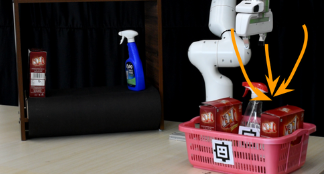
\includegraphics[width=3.1cm]{Figures/intro_frames/teach1.png}};
\node[photo, right=1.5mm of t1] (t2) {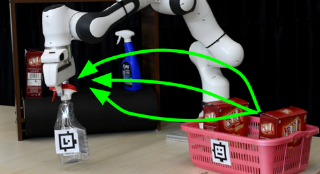
\includegraphics[width=3.1cm]{Figures/intro_frames/teach2.png}};
\node[photo, right=1.5mm of t2] (t3) {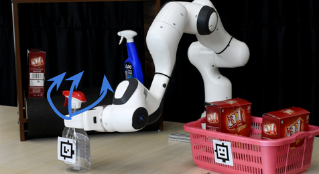
\includegraphics[width=3.1cm]{Figures/intro_frames/teach3.png}};
\node[photo, right=1.5mm of t3] (t4) {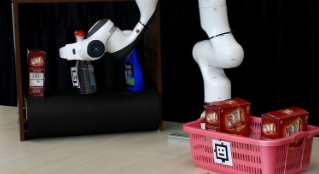
\includegraphics[width=3.1cm]{Figures/intro_frames/teach4.png}};
\node[quote, below=0.5mm of t1] {``grasping from top''};
\node[quote, below=0.5mm of t2] {``placing on table''};
\node[quote, below=0.5mm of t3] {``grasping from side''};
\node[quote, below=0.5mm of t4] {``placing on shelf''};
\node[banner, tli] at ([xshift=-1mm,yshift=3.5mm]t1.north west)
  {\faUser~1.\ Expert teaches: narrated, segmented demonstrations};
\begin{scope}[on background layer]
  \node[fill=teachbg, rounded corners, inner sep=2.5mm,
        fit=(t1)(t4), yshift=-1mm, minimum height=2.6cm] (teachbox) {};
\end{scope}
% ---------- (2) Query ----------
\node[photo, below=13mm of t1.south west, anchor=north west] (q1a)
  {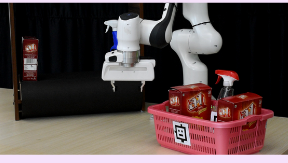
\includegraphics[width=2.75cm]{Figures/intro_frames/query1a.png}};
\node[photo, right=4mm of q1a] (q1b) {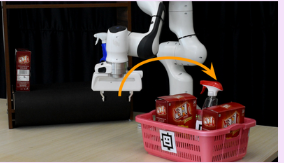
\includegraphics[width=2.75cm]{Figures/intro_frames/query1b.png}};
\node[photo, right=7mm of q1b] (q2a) {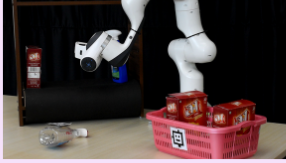
\includegraphics[width=2.75cm]{Figures/intro_frames/query2a.png}};
\node[photo, right=4mm of q2a] (q2b) {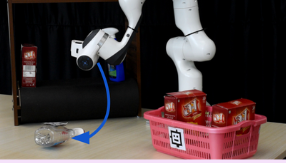
\includegraphics[width=2.75cm]{Figures/intro_frames/query2b.png}};
\draw[->, thick] (q1a) -- (q1b);
\draw[->, thick] (q2a) -- (q2b);
\node[quote, below=0.5mm of q1b.south west, anchor=north] at ([xshift=-3mm]q1b.south west|-q1b.south)
  {};
\node[quote] at ([yshift=-2.5mm]$(q1a.south)!0.5!(q1b.south)$) {\faUser~``I would grasp from top''};
\node[quote] at ([yshift=-2.5mm]$(q2a.south)!0.5!(q2b.south)$) {\faUser~``I would grasp from side''};
\node[banner, tli] at ([xshift=-1mm,yshift=3.5mm]q1a.north west)
  {\faRobot~2.\ Robot queries the situations it is uncertain about};
\begin{scope}[on background layer]
  \node[fill=querybg, rounded corners, inner sep=2.5mm,
        fit=(q1a)(q2b), yshift=-1mm, minimum height=2.6cm] (querybox) {};
\end{scope}
% ---------- (3) Test ----------
\node[photo, right=8mm of t4.north east, anchor=north west, yshift=-9mm] (test)
  {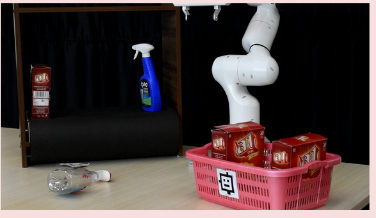
\includegraphics[width=4.1cm]{Figures/intro_frames/test.png}};
\node[banner, tli, text width=4.1cm, align=left] at ([xshift=-1mm,yshift=6mm]test.north west)
  {\faBolt~3.\ Test: perturbation};
\node[font=\scriptsize, align=center, below=1.5mm of test]
  (testtxt) {bottle knocked over $\rightarrow$ localizer\\ detects mode change $\rightarrow$\\ ``grasp from side'' engaged\\ \textbf{failure avoided}};
\begin{scope}[on background layer]
  \node[fill=testbg, rounded corners, inner sep=2.5mm, fit=(test)(testtxt)] {};
\end{scope}
\end{tikzpicture}%
}
\caption{\textbf{Teaching, querying, and recovery on the restocking task.} (1) The expert demonstrates the full task, marking each subtask with a trigger signal while narrating. (2) The trained classifier identifies the physical situations where its guard estimate is most uncertain and asks the expert what mode should be executed from them; the answers are short, safe sub-demonstrations. (3) At test time the memory-less localizer detects a perturbation-induced mode change from the instantaneous state and engages the appropriate skill.}
\label{fig:intro}
\end{figure*}
\section{Introduction}
Long-horizon manipulation is commonly addressed by decomposing a task into subtasks with associated skills~\cite{dalal2024manipgen,Ahn2022DoAI,wu2023tidybot,huang2022inner,merging_dmp}, each learned via reinforcement or imitation learning. Yet real-world execution introduces physical perturbations that can induce \emph{task-level} failures even when the low-level motion policy executes flawlessly. Consider a robot scooping rice from a bowl, transporting it, and depositing it onto a plate: an external disturbance that jostles the arm mid-transport merely deflects the path---from which a motion policy such as a Dynamic Movement Primitive~\cite{Ijspeert_NC_2013} can spatially recover---but a disturbance that tips the spoon and slides the rice off is a \emph{task-level} failure: the arm still reaches the deposit location, on schedule, carrying nothing. Reaching the target does not resolve it. Robust manipulation therefore demands reactivity at both the motion \emph{and} the task level.

We adopt the well-established view that task-level reactivity is naturally expressed as a \emph{hybrid automaton}: the joint robot--environment state space is partitioned into discrete \emph{modes} (here, \textit{Scoop}, \textit{Transport}, \textit{Deposit}), each mode selecting an active skill, with transitions governing the sequencing. Two properties make such an automaton robust to perturbation. \emph{Goal reachability} ensures each skill drives the state to the next transition boundary, guaranteeing task progress; \emph{mode invariance} ensures the state remains within a mode until that boundary---e.g., that the rice remains loaded on the spoon throughout \textit{Transport}---so that an unexpected departure from a mode is precisely a task-level failure signal. Temporal-logic imitation (TLI)~\cite{wang2022temporal} makes these conditions explicit and, when they hold for the learned per-mode policies, guarantees that any admissible discrete plan is realized by the continuous system.

Crucially, in this formalism the discrete modes are only labels; the semantic content and the robustness both reside in the \emph{transitions} and in the function that grounds continuous state to modes. We call this the \emph{localization function} $L:\mathcal{X}\!\to\!\mathcal{M}$. For our scooping robot, $L$ must decide, from signals such as the spoon-tilt angle and a contact/load reading, which of $\{$\textit{Scoop}, \textit{Transport}, \textit{Deposit}$\}$ is currently active---and, implicitly, exactly where the boundary between them, the \emph{guard}, lies in that feature space. Given the automaton, runtime reactivity reduces entirely to this: localize the current state onto the correct side of the guard, at every control step. The automaton itself is easy to write down; the guard is where the difficulty lives. The central question of this paper is therefore \emph{how the guard is obtained}, and at what cost in expertise, data, and safety (Fig.~\ref{fig:seal_ltl_comp}).

The classical answer, exemplified by TLI, is to place the guard by hand (Fig.~\ref{fig:seal_ltl_comp}, bottom left): an expert authors it analytically, reasoning from a physical model of the task---rice mass, spoon geometry, expected sensor range---to a rule such as ``a load reading below 0.5\,N while tilt exceeds $20^\circ$ means \textit{Transport} has failed.'' This consumes no data at all; the guard is placed by expertise alone, and its accuracy is bounded by how well the expert's analytic model matches the true sensor and task distribution. If real load-cell noise, rice clumping, or spoon-to-grain friction deviate from that model---as they generally do---the guard is simply in the wrong place, and no amount of subsequent operation corrects it, because no data was ever consulted in placing it. Hand-designed grounding is thus brittle to observation noise (Sec.~\ref{sec:scooping}) not for lack of engineering effort, but by construction.

GLiDE~\cite{wang2024grounding} recognizes exactly this mismatch and fits the guard to data instead of asserting it (Fig.~\ref{fig:seal_ltl_comp}, bottom center). It perturbs demonstrations---tilting the spoon further, jostling the arm---replays them, and uses an automatic success/failure oracle together with a reset mechanism to label thousands of rollouts, then fits the mode boundaries to the resulting cloud of successes and failures. The guard now hugs the real distribution rather than an idealized model of it. But tracing the boundary this way requires \emph{inducing} the failure, repeatedly and at volume: to learn where rice falls off the spoon, GLiDE must spill rice, thousands of times, in an environment that can automatically detect the spill and reset it. For contact-rich tasks this is precisely the regime that does not exist---grains cannot be un-spilled, payloads cannot be un-dropped, and a deployed system exists to avoid these outcomes, not to rehearse them.

The two state-of-the-art answers thus sit at uncomfortable extremes: TLI needs no data but inherits every error of the expert's analytic model, while GLiDE fixes the model error only by consuming failure data that is unsafe, expensive, or physically impossible to collect. What is missing is a way to fit the guard to the \emph{real} distribution---retaining GLiDE's data-driven accuracy---using only data that is safe to produce. This is the gap SEAL fills: a handful of safe, human-segmented demonstrations gives an initial estimate of the guard, and a small number of additional safe demonstrations, actively requested at the specific states where that estimate is least certain, sharpen it to the precision that would otherwise demand a cloud of failures (Fig.~\ref{fig:seal_ltl_comp}, bottom right; pipeline in Fig.~\ref{fig:intro}). No rice is ever spilled to learn where it would spill.

\textbf{Approach.} SEAL retains the designed automaton and learns its localization function---never requiring resets, self-supervised rollouts, or failure data. An LLM proposes a compact set of spatially invariant features from the task description, and an information-theoretic check certifies that the modes are actually separable in that space before any learning begins. A Gaussian Process Classifier trained on the segmented demonstrations then serves as the localizer; its epistemic uncertainty pinpoints the states at which the guard estimate is weakest, and these states become the active demonstration requests. At runtime the localizer reads the instantaneous physical state (the current tilt and load reading, not the history of modes visited), so a perturbation that drives the state across a mode boundary is registered within a control step and recovery is triggered---regardless of where the nominal plan believes the task to be. Because the classifier's confidence is calibrated, transitions are accepted only when confident and persistent, decoupling switching latency from the false-positive rate.



\textbf{Contributions.}
\begin{enumerate}
\item \textbf{Safe localization from success-only demonstrations.} We formulate reactive sequencing as learning the localization function of a known automaton from safe data alone, and provide a two-stage feature-engineering pipeline that pairs an LLM semantic prior with an information-theoretic \emph{observability certificate}, yielding a minimal, spatially invariant space in which modes are instantaneously separable.
\item \textbf{Uncertainty-targeted active querying.} A Gaussian Process Classifier exposes epistemic uncertainty that directs expert effort to under-determined guard regions---without perturbations, resets, or failure data---and the same signal extends naturally to invariance/reachability-driven guard refinement against the true closed-loop dynamics.
\item \textbf{Confidence-gated switching.} We exploit the classifier's calibrated confidence to achieve low switching latency and a low false-positive rate simultaneously---a trade-off that hand-tuned automata and uncalibrated groundings must instead resolve with long debounce windows.
\item \textbf{Extensive validation} across five simulated and real-world contact-rich tasks and a 10-participant user study, including an empirical certification of goal reachability and mode invariance on the learned regions.
\end{enumerate}

%%%%%%%%%%%%%%%%%%%%%%%%%%%%%%%%%%%%%%%%%%%%%%%%%%%%%%%%%%%%%%%%%%%%%%%%%%%%%%%%
\section{Related Work}
\textbf{Failure detection and runtime monitoring.} Failure detection in manipulation is largely treated either as anomaly/out-of-distribution (OOD) detection using statistical models or as supervised/self-supervised learning on high-dimensional data. In the first setting, Eiband \emph{et al.}~\cite{eiband_intuitive_2019} and Willibald \emph{et al.}~\cite{willibald_collaborative_2020} model successful demonstration features and their time-steps as a Gaussian Mixture Model and flag failures via a Mahalanobis-distance threshold to the time-conditioned nominal trajectory; \cite{hierarchical} conditions on end-effector pose rather than time, arguing that interaction dynamics dominate; and \cite{10.5555/3398761.3398779} fits a Hidden Markov Model and detects anomalies online by comparing observation distributions within a sliding window. These methods are effective but share two limitations: an OOD observation does not imply an impending failure, and time-conditioned nominal profiles do not transfer under spatial perturbation, precluding spatial generalization. More recent post-hoc detectors learn distance metrics with time-varying thresholds~\cite{xu_can_2025}, combine a VLM with temporal action consistency~\cite{agia2024unpacking}, or measure action-chunk entropy and observation novelty via random network distillation~\cite{romer2025fiper}. Action-consistency signals are powerful but presuppose action-chunking policies such as diffusion policy~\cite{chi2024diffusionpolicy} or ACT~\cite{Zhao-RSS-23}; SEAL, in contrast, supervises \emph{any} policy, including pre-programmed skills. A parallel line uses VLMs for monitoring and recovery~\cite{sinha_real-time_2024,etukuru_robot_2024,elhafsi_semantic_2023,du_vision-language_2023,zhang_grounding_2023,pacaud_guardian_2025,agia2024unpacking}, but these either fine-tune on failure datasets or query the VLM intermittently due to latency; we use an LLM only at training time and monitor at upwards of 30\,Hz with a lightweight classifier. In the supervised setting, \cite{9636455} trains a deep multimodal classifier on failure examples, Sliwowski and Lee~\cite{sliwowski_conditionnet_2025} predict action phase and flag phase mismatches, and \cite{11245878} selects among detectors by confidence. Their reliance on failure demonstrations makes them unsuitable when such data is unsafe or hard to collect---precisely the regime SEAL targets.

\textbf{Mode grounding and precondition learning.} Estimating the semantic mode from observations may be unsupervised (modes discovered) or supervised (modes defined). Unsupervised approaches segment trajectories by geometric reconstruction error~\cite{shi2023waypointbased} or by inverse RL and feature clustering~\cite{hierarchical}. Among supervised approaches, Eiband \emph{et al.}~\cite{eiband_online_2023} combine symbolic and data-driven skill recognition but need hand-specified pre/post-conditions or many per-skill examples; Hegemann \emph{et al.}~\cite{hegemann_learning_2022} ground sensor values with binary predicates fed to a decision tree; and \cite{9811675} composes predicate classifiers with Bayesian state estimation. Purely predicate-based grounding requires an expert to design and train predicates per task; SEAL instead learns the grounding directly and supports both predicate and continuous observations. A related line, initiated by Konidaris \emph{et al.}~\cite{konidaris2018skills}, learns symbolic representations---initiation sets and effect distributions of skills---from interaction data for high-level \emph{planning}; SEAL learns the analogous regions jointly, but from safe demonstrations alone and for a different purpose: real-time localization and failure monitoring during execution rather than offline symbol construction. Finally, \cite{sliwowski_m2r2_2025} learns multimodal representations for temporal action segmentation~\cite{TAS}, and \cite{shah2022value} learns state representations from skill value functions; these are complementary representation learners that could feed a runtime localizer such as ours.

\textbf{Interactive and active imitation learning.} SEAL's querying mechanism belongs to the tradition of robots that solicit targeted help from a human teacher. Chernova and Veloso~\cite{chernova2009confidence} gate autonomous execution on classifier confidence and request demonstrations in low-confidence states; Cakmak and Thomaz~\cite{cakmak2012designing} study which query types make such requests effective for human teachers. The DAgger family formalizes iterative expert correction~\cite{ross2011dagger}, with SafeDAgger~\cite{zhang2017safedagger} and EnsembleDAgger~\cite{menda2019ensembledagger} invoking the expert only where a learned policy is unreliable or an ensemble disagrees. All of these query at the \emph{action} level to improve a control policy, and their queries arise during (possibly unsafe) autonomous rollouts. SEAL transfers the query-when-uncertain principle to the \emph{task} level: queries are short, prescriptive, segmented demonstrations that ground a known automaton, they are generated offline from the calibrated epistemic uncertainty of a GPC rather than from ensemble disagreement, and answering them never requires the robot to act in an uncertain state.

\textbf{Automaton-based sequencing: from funnels to learned grounding.} The formal backbone of our setting is classical: sequential composition~\cite{burridge1999sequential} showed that goal-directed controllers whose attractors lie in the domain of the next controller compose into robust long-horizon behavior (our Assumption~\ref{as:prim} is exactly this condition), and reactive synthesis~\cite{kressgazit2009temporal} showed how temporal-logic specifications compile into correct-by-construction hybrid controllers---assuming the discrete state can be sensed. Temporal Logic Imitation (TLI)~\cite{wang2022temporal} brought this program to learning-from-demonstration: it specifies admissible transitions via an LTL formula and proves that, if each learned dynamical-system policy satisfies mode invariance and goal reachability, any admissible plan is realized robustly---its grounding, however, is a hand-engineered sensor model. GLiDE~\cite{wang2024grounding} closes this gap by \emph{learning} the grounding: it takes valid transitions from an LLM feasibility matrix and learns mode boundaries by perturbing demonstrations and checking, via an outcome oracle and resets, which perturbed trajectories still succeed. Both are important precedents, and we adopt their central abstraction. We differ in \emph{how the grounding is obtained}: SEAL learns it from a few segmented expert demonstrations with minimal post-processing, avoiding (i) perturbation strategies that must be designed per task, (ii) an environment that resets autonomously, and (iii) an outcome oracle. This is a more realistic setting for demonstrators who are proficient in the task but not in model design, and it is the only one of the three that applies when failures are unsafe to induce. We further show (Sec.~\ref{sec:scooping}) that calibrated confidence lets SEAL suppress spurious transitions without incurring switching latency---a property that neither a hand-tuned automaton nor an uncalibrated grounding provides. We do not compare against TAMP frameworks, which plan over tasks and motions rather than reactively sequencing over a fixed nominal plan; when such frameworks incorporate recovery, they typically replan or rely on the anomaly/VLM detectors discussed above.

%%%%%%%%%%%%%%%%%%%%%%%%%%%%%%%%%%%%%%%%%%%%%%%%%%%%%%%%%%%%%%%%%%%%%%%%%%%%%%%%
\section{Problem Formulation}
\label{sec:formulation}

\subsection{Task Model}
We model the task as a hybrid automaton $H=(\mathcal{M},\mathcal{X}_{\min},\{R_m\},\{\pi_m\},S)$, where $\mathcal{M}$ is a finite set of modes (subtasks), $\mathcal{X}_{\min}$ is a reduced continuous feature space (Sec.~\ref{sec:feature_engineering}), $R_m\subseteq\mathcal{X}_{\min}$ is the region in which mode $m$ is the correct mode to execute, $\pi_m$ is the skill (a goal-directed dynamical system) executed in mode $m$, and $S=(m_1,\dots,m_K)$ is a nominal mode sequence given by task design. The regions $\{R_m\}$ partition $\mathcal{X}_{\min}$; the boundary between adjacent regions defines a \emph{guard} $G_{m,m'}=\partial R_m\cap\partial R_{m'}$, and crossing a guard is a mode transition. The granularity of the segmentation into modes is a design choice, constrained only by Assumptions~\ref{as:obs}--\ref{as:prim} below.

The partition induces the \emph{true localization function}
\begin{equation}
L:\ \mathcal{X}_{\min}\to\mathcal{M},\qquad L(\mathbf{x})=m \iff \mathbf{x}\in R_m ,
\end{equation}
which reports, for any physical state, the mode that should currently be executing. $L$ is exactly the object all grounding methods construct (Fig.~\ref{fig:seal_ltl_comp}): learning $L$ \emph{is} learning the partition $\{R_m\}$---the same object that TLI places by hand and GLiDE fits from perturbed rollouts. SEAL learns an estimator
\begin{equation}
f(\mathbf{x})=\arg\max_{m}\,P(m\mid\mathbf{x}),
\end{equation}
where $P(m\mid\mathbf{x})$ is the posterior of the Gaussian Process Classifier of Sec.~\ref{sec:gpc}. The decision surfaces of $f$ are its \emph{learned guards}; the learning problem of this paper is to make them match the true guards using only safe data.

\subsection{Robustness Properties and Assumptions}
We recall the two properties from~\cite{wang2022temporal} that govern robustness, stated here on the reduced feature space in which the localizer operates.

\begin{definition}[Mode invariance]
\label{def:inv}
A policy $\pi_m$ with nominal successor $m'$ is \emph{invariant} on $R_m$ if every feature trajectory it induces from $\mathbf{x}\in R_m$ remains in $R_m$ until it reaches the nominal guard $G_{m,m'}$. Exiting $R_m$ through any other boundary is an \emph{invariance violation}---the task-level failure event we must detect.
\end{definition}

\begin{definition}[Goal reachability]
\label{def:reach}
A policy $\pi_m$ is \emph{goal-reaching} for the transition $m\!\to\!m'$ if it drives the feature state into the guard $G_{m,m'}$ (equivalently, its attractor lies in the initiation set of $m'$).
\end{definition}

Two assumptions make the problem well-posed. The first is what allows a \emph{memory-less} localizer to succeed at all.

\begin{assumption}[Instantaneous observability]
\label{as:obs}
The mode is identifiable from the instantaneous feature vector: $L$ is well-defined on $\mathcal{X}_{\min}$, i.e., the regions $\{R_m\}$ do not overlap. Operationally, we certify this by requiring the joint mutual information between features and labels to approach the label entropy, $I(X_{\min};Y)\approx H(Y)$ (Sec.~\ref{sec:feature_engineering}).
\end{assumption}

\begin{remark}[Scope of the certificate]
\label{rem:scope}
The MI certificate is estimated on the \emph{demonstrated} distribution, so it certifies separability on the support of the demonstrations, not on all of $\mathcal{X}_{\min}$. Perturbations, however, drive the state into precisely the regions demonstrations never visit. Closing this gap---extending the region on which $f$ agrees with $L$ beyond the initial demonstrations, using only safe data---is the role of uncertainty-targeted active querying (Sec.~\ref{sec:active}).
\end{remark}

\begin{assumption}[Primitive competence]
\label{as:prim}
Each primitive $\pi_m$ is a goal-directed dynamical system whose attractor lies in the initiation set of its successor~\cite{burridge1999sequential}. Geometric mode invariance and goal reachability thus hold \emph{by construction}. The residual, physical component of invariance (e.g., ``payload retained'') is not controllable by $\pi_m$ and is precisely what we monitor.
\end{assumption}

\subsection{Closed-Loop Behavior}
Under these assumptions the localizer plays a dual role, which we make explicit.

\begin{proposition}[Localization determines closed-loop sequencing]
\label{prop:main}
Let Assumptions~\ref{as:obs}--\ref{as:prim} hold, and suppose $f=L$ at every state visited by the closed-loop system. Then the mode trajectory of $H$ is determined by the guard crossings of $f$: (i) along nominal execution, each $\pi_m$ drives the state into $G_{m,m'}$ and the task completes; (ii) upon a physical invariance violation, the state exits $R_m$ through a non-nominal boundary into some region $R_k$, $f$ re-localizes to $k$, and $\pi_k$ is engaged.
\end{proposition}

\begin{proof}[Proof sketch]
Case (i): by Assumption~\ref{as:prim}, from any $\mathbf{x}\in R_m$ the flow of $\pi_m$ reaches $G_{m,m'}$ without leaving $R_m$; since $f=L$, the transition fires exactly at the crossing, and induction over $S$ completes the task. Case (ii): a physical violation moves the state into some $R_k$ with $k\neq m'$; since the regions partition $\mathcal{X}_{\min}$ and $f=L$, $f$ outputs $k$, and execution continues from $R_k$ per case (i).
\end{proof}

The hypothesis $f=L$ on the visited states is the crux: it holds where data has constrained $f$, and fails where it has not (Remark~\ref{rem:scope}).

\begin{remark}[Capacity is not the bottleneck; coverage is]
\label{rem:consistency}
Instantiating $f$ as a Gaussian Process Classifier with a universal kernel~\cite{steinwart2001influence} makes it Bayes-consistent: $f\to L$ as labeled data accumulates \emph{on the support of the data-generating distribution}. Universality, however, guarantees nothing off-support---no model capacity can place a guard in a region no demonstration has visited. The GPC contributes the missing half operationally: its epistemic variance is a quantitative surrogate for the set where the hypothesis $f=L$ may fail, and the acquisition function of Sec.~\ref{sec:active} queries exactly there, converting uncovered states into covered ones with safe demonstrations.
\end{remark} The paper's algorithmic content is therefore aimed at enlarging the region where the hypothesis holds---safely---and Sec.~\ref{sec:experiments} certifies it empirically by measuring invariance-violation and reachability-success rates on the learned regions. In deployment, Algorithm~\ref{alg:supervision} additionally relaxes the idealized instantaneous-crossing rule: a transition is accepted only when it is confident and persistent, which trades an adjustable dwell time against robustness to observation noise near guards.

Proposition~\ref{prop:main} clarifies the division of labor: reachability (Assumption~\ref{as:prim}) supplies task progress and completion, while the learned $f$ serves as a \emph{data-driven invariance monitor}, replacing TLI's hand-engineered sensor model. The remainder of the paper concerns learning $f$ safely and efficiently.

%%%%%%%%%%%%%%%%%%%%%%%%%%%%%%%%%%%%%%%%%%%%%%%%%%%%%%%%%%%%%%%%%%%%%%%%%%%%%%%%
\section{Method}
SEAL executes the program laid out by Sec.~\ref{sec:formulation}: construct a feature space in which Assumption~\ref{as:obs} verifiably holds (Sec.~\ref{sec:feature_engineering}), learn the estimator $f$ with a model whose uncertainty reports where $f=L$ may fail (Sec.~\ref{sec:gpc}), enlarge that region with safe, targeted queries (Sec.~\ref{sec:active}), and deploy $f$ as a runtime invariance monitor over the primitives (Sec.~\ref{sec:supervision}). Fig.~\ref{fig:framework} summarizes the pipeline.

\begin{figure*}[t]
\centering
% TikZ scaffold; thumbnails in Figures/framework_frames/ are LOW-RES CROPS of the
% old framework.png -- regenerate from the original matplotlib outputs (same
% filenames) for print quality. Prompt-template text moved to Appendix~B.
\resizebox{\textwidth}{!}{%
\begin{tikzpicture}[font=\small, >=Latex,
  photo/.style={inner sep=1pt, draw=gray!40, thin},
  blk/.style={rounded corners, draw, thick, align=center, inner sep=3pt,
              minimum height=8mm, font=\small},
  lbl/.style={font=\scriptsize, align=center},
  panel/.style={font=\small\bfseries, anchor=west},
]
% =============== (a) feature engineering (top) ===============
\node[blk, text width=24mm] (prompt)
  {task prompt\\ \scriptsize(Appendix~\ref{app:feature})};
\node[blk, right=8mm of prompt] (llm) {LLM};
\node[blk, right=8mm of llm, text width=22mm] (fsel) {candidate\\ features $F_{\text{sel}}$};
\node[blk, right=8mm of fsel, text width=30mm] (mi)
  {sufficiency check\\ $I(X_{\text{sel}};Y)\ge(1-\epsilon)I(X_{\text{raw}};Y)$};
\node[blk, right=8mm of mi, text width=26mm] (minz)
  {MI minimization:\\ drop redundant\\ features};
\node[blk, right=8mm of minz, fill=teachbg, text width=20mm] (fmin)
  {$F_{\min}$, $\mathcal{X}_{\min}$\\ \scriptsize fixed for all rounds};
\draw[->, thick] (prompt) -- (llm);
\draw[->, thick] (llm) -- (fsel);
\draw[->, thick] (fsel) -- (mi);
\draw[->, thick] (mi) -- node[above, font=\scriptsize]{pass} (minz);
\draw[->, thick] (minz) -- (fmin);
\draw[->, thick, dashed] (mi.south) -- ++(0,-4.5mm) -| node[below, pos=0.25, font=\scriptsize]
  {fail: user refines task description} (prompt.south);
\node[panel] at ([xshift=-2mm,yshift=4mm]prompt.north west)
  {(a) Two-stage feature engineering = observability certificate for Assumption~\ref{as:obs} (Sec.~\ref{sec:feature_engineering})};
% =============== (b) active learning loop (bottom) ===============
\node[photo, below=17mm of prompt.south west, anchor=north west] (demos) {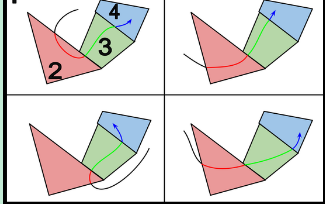
\includegraphics[height=2.1cm]{Figures/framework_frames/demos.png}};
\node[photo, right=13mm of demos] (weak) {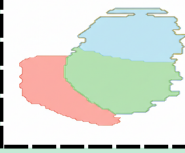
\includegraphics[height=2.1cm]{Figures/framework_frames/weak.png}};
\node[photo, right=13mm of weak] (uncert) {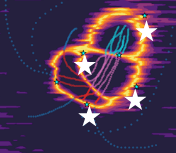
\includegraphics[height=2.1cm]{Figures/framework_frames/uncert.png}};
\node[photo, right=13mm of uncert] (queried) {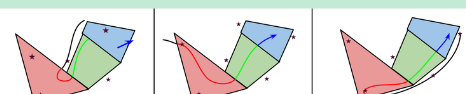
\includegraphics[height=1.35cm]{Figures/framework_frames/queried.png}};
\node[photo, right=13mm of queried] (strong) {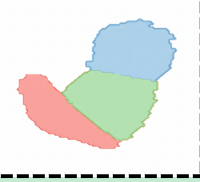
\includegraphics[height=2.1cm]{Figures/framework_frames/strong.png}};
\node[lbl, below=1mm of demos]  {initial segmented\\ demos $\mathcal{D}_0$};
\node[lbl, below=1mm of weak]   {weak classifier};
\node[lbl, below=1mm of uncert] {acquisition $\alpha$,\\ query points $X_K$};
\node[lbl, below=1mm of queried]{safe demos through $X_K$};
\node[lbl, below=1mm of strong] {strong classifier $f$};
\draw[->, thick] (demos) -- node[above, font=\scriptsize]{train} (weak);
\draw[->, thick] (weak) -- (uncert);
\draw[->, thick] (uncert) -- node[above, font=\scriptsize]{\faUser} (queried);
\draw[->, thick] (queried) -- node[above, font=\scriptsize]{retrain} (strong);
\node[panel] at ([xshift=-2mm,yshift=5mm]demos.north west)
  {(b) Active learning of the localizer (Algorithm~\ref{alg:active})};
\end{tikzpicture}%
}
\caption{\textbf{The SEAL pipeline.} (a) An LLM proposes candidate features from the task description; a mutual-information sufficiency check accepts them only if no mode-relevant information was discarded (else the user refines the description), and a minimization pass drops redundant features. The resulting $F_{\min}$ is fixed for all subsequent rounds and at test time. (b) In $F_{\min}$, the initial segmented demonstrations train a weak localizer; the acquisition score selects the states where the guard estimate is least certain, the expert supplies safe demonstrations through them, and retraining yields the deployed localizer $f$ (thumbnails: 2D navigation task of Sec.~\ref{sec:2d_nav}).}
\label{fig:framework}
\end{figure*}

\subsection{Initial Expert Demonstrations}
An expert provides a set of initial demonstrations of the complete task in the raw feature space, yielding $\mathcal{D}_{0,\text{raw}}$. A trajectory is a sequence of feature states $\tau=\{\mathbf{x}_t\}_{t=1}^{T}$, and the expert supplies dense, per-point mode labels by emitting a trigger signal upon completion of each subtask. Once the minimal feature set $F_{\min}$ is determined (Sec.~\ref{sec:feature_engineering}), the raw data is processed into a working dataset of $N$ labeled trajectories,
\begin{equation}
\mathcal{D}_{0,\text{min}}=\{(\tau_i,\ell_i)\}_{i=1}^N
\;\equiv\;\bigcup_{i=1}^{N}\bigcup_{t=1}^{T_i}\{(\mathbf{x}_{i,t},m_{i,t})\},
\end{equation}
where $\ell_i=\{m_{i,t}\}_{t=1}^{T_i}$ are the per-point mode labels and the right-hand side is the flattened point set on which the classifier trains. These demonstrations are not overhead specific to the classifier: being successful expert trajectories, they can double as training data for the low-level primitives. (To isolate the mode supervisor, our experiments use programmatic primitives.) The only additional cost is the per-segment trigger signal, which we validate as negligible in Sec.~\ref{sec:user_study}. We assume all initial demonstrations adhere to valid transitions and complete the task successfully.

\subsection{Two-Stage Feature Engineering as an Observability Certificate}
\label{sec:feature_engineering}
The localizer must operate in a space where every sampled point is physically realizable and interpretable for expert labeling; a sample drawn in raw pixel space is neither. We therefore work with grounded features (object poses, relations). However, even a few absolute object poses push the dimension above ten, which is problematic for two reasons: the curse of dimensionality inflates the demonstrations needed for dense coverage, and the physically valid manifold occupies a vanishing fraction of the ambient space, so uncertainty-driven sampling (Sec.~\ref{sec:active}) frequently proposes infeasible configurations (objects suspended in mid-air) that an expert cannot demonstrate. We reduce the space with a two-stage pipeline (Fig.~\ref{fig:framework}a) that also \emph{certifies} Assumption~\ref{as:obs}.

\textbf{Stage 1: Semantic generation.} An LLM~\cite{gemini} acts as a semantic prior. Prompted with the task description, available raw features $F_{\text{raw}}$, and target modes, it outputs a candidate set $F_{\text{sel}}$ that penalizes absolute coordinates in favor of spatially invariant relative metrics. We map the demonstrations into $X_{\text{sel}}$ and estimate the joint mutual information $I(X_{\text{sel}};Y)$ against the discrete mode labels $Y$ using a $k$-nearest-neighbor estimator for mixed continuous--discrete data~\cite{10.1371/journal.pone.0087357}. If $I(X_{\text{sel}};Y)$ falls short of the raw baseline $I(X_{\text{raw}};Y)\approx H(Y)$ by more than a tolerance $\epsilon$ (we accept when $I(X_{\text{sel}};Y)\ge(1-\epsilon)\,I(X_{\text{raw}};Y)$, $\epsilon=\todo{state $\epsilon$ used}$), the LLM has discarded mode-relevant information; the system rejects $F_{\text{sel}}$ and asks the user for a more detailed description. This test is exactly the empirical observability certificate of Assumption~\ref{as:obs}.

\textbf{Stage 2: Mathematical minimization.} Given a sufficient $F_{\text{sel}}$, we prune redundancy by evaluating lower-dimensional projections---dropping feature columns and recomputing the MI---and define $X_{\min}$ as the lowest-dimensional projection that preserves the baseline MI, with corresponding features $F_{\min}$. If no feature is redundant, $F_{\min}=F_{\text{sel}}$. Because MI alone cannot distinguish causal geometry from spurious spatial correlation in the few-shot regime (Appendix~\ref{app:feature}), the LLM's invariance prior is what makes the resulting space causally robust; MI supplies the sufficiency and minimality guarantees. In all later rounds, new data is processed directly into $F_{\min}$.

\subsection{Localization via a Gaussian Process Classifier}
\label{sec:gpc}
We instantiate $f$ as a Gaussian Process Classifier (GPC) for its calibrated, decomposable uncertainty, which is central both to active learning and to confidence-gated switching. A GPC defines a distribution over latent functions; the posterior predictive for a test point $\mathbf{x}^*$ is
\begin{equation}
P(m\mid\mathbf{x}^*,\mathcal{D}_{k})=\int\sigma(f^*)\,p(f^*\mid\mathcal{D}_{k})\,df^*,
\end{equation}
with $\sigma(\cdot)$ the softmax link and $p(f^*\mid\mathcal{D}_{k})$ the (non-Gaussian) latent predictive distribution. The integral is intractable, so we approximate the posterior by a Gaussian $q(\mathbf{f})$ via variational inference using GPyTorch~\cite{gardner2018gpytorch} with $M=\todo{state \# inducing points}$ inducing points; a calibration analysis of the resulting confidences is given in Appendix~\ref{app:ablation}.

\textbf{Mixed continuous--discrete features.} Robotic states mix continuous variables $\mathbf{x}_{\text{cont}}\in\mathbb{R}^d$ (relative distances) with discrete ones $c\in\mathbb{N}$ (e.g., gripper status). A single RBF kernel over the joint space assumes context-independent correlation, while separate classifiers per discrete value waste data. We use a product kernel
\begin{equation}
k(\mathbf{x},\mathbf{x}')=k_{\text{RBF}}(\mathbf{x}_{\text{cont}},\mathbf{x}'_{\text{cont}})\cdot k_{\text{idx}}(c,c'),
\end{equation}
where the index kernel $k_{\text{idx}}$ learns a low-rank covariance $\mathbf{B}$ across discrete contexts. Unlike a fixed Kronecker delta, a learnable $\mathbf{B}$ lets the GPC share information across contexts when useful or isolate them when not, and it scales to more than two discrete contexts where per-context models become data-hungry (Appendix~\ref{app:ablation}). During candidate selection we fix the discrete variables and sample the continuous space.

\subsection{Uncertainty-Targeted Active Learning}
\label{sec:active}
The GPC exposes \emph{epistemic} uncertainty---ignorance in low-density regions---distinct from \emph{aleatoric} boundary ambiguity. As a proxy we use the summed latent variance across modes, which is large wherever data is sparse (though it does not separate the two sources perfectly near guards),
\begin{equation}
\eta(\mathbf{x}^*)=\sum_{m\in\mathcal{M}}\text{Var}(f^*_m).
\end{equation}
Because raw epistemic uncertainty peaks at the extreme edges of the state space, we weight it by a centring prior $W(\mathbf{x}^*)$, a Gaussian over the workspace whose mean and covariance are set once from the spread of $\mathcal{D}_{0}$ (not tuned per task). The acquisition score is
\begin{equation}
\alpha(\mathbf{x}^*)=\eta(\mathbf{x}^*)\cdot W(\mathbf{x}^*).
\end{equation}
The learning loop is summarized in Algorithm~\ref{alg:active} and illustrated in Fig.~\ref{fig:framework}b. Batch diversity uses greedy furthest-point sampling on standardized features (so that meters, radians, and binary flags are comparable),
\begin{equation}\label{eq:sampling}
\mathbf{x}_k=\operatorname*{argmax}_{\mathbf{x}\in\mathcal{U}_{\text{top}}\setminus X_{k-1}}\ \min_{\mathbf{x}_j\in X_{k-1}}\|\mathbf{x}-\mathbf{x}_j\|_2,
\end{equation}
initialized at $\mathbf{x}_1=\arg\max_{\mathbf{x}}\alpha(\mathbf{x})$. The candidate grid is feasible precisely because Sec.~\ref{sec:feature_engineering} has reduced the space to a few dimensions. Because the features are grounded (object poses, relations), each queried point is realized physically: the scene is configured to match the queried feature state (e.g., the spray bottle is laid on its side at the queried offset), and the expert demonstrates from there, supplying \emph{prescriptive} labels---the mode that should be executed from that state to advance the task. Our experiments use a single active round.

\begin{algorithm}
\caption{Uncertainty-Targeted Active Learning}\label{alg:active}
\begin{algorithmic}[1]
\Require initial demos $\mathcal{D}_{0}$, batch size $K$, rounds $R$
\For{$k=0,\dots,R-1$}
\State train GPC $f$ on $\mathcal{D}_{k}$
\State compute $\alpha(\mathbf{x})=\eta(\mathbf{x})\,W(\mathbf{x})$ on a dense grid over the bounding box of $\mathcal{D}_{0}$
\State $\mathcal{U}_{\text{top}}\gets$ top decile of $\alpha$
\State $X_K\gets K$ diverse points from $\mathcal{U}_{\text{top}}$ via Eq.~\eqref{eq:sampling}
\State configure scenes at $X_K$; expert provides safe, segmented demos $\mathcal{D}_{\text{new}}$
\State $\mathcal{D}_{k+1}\gets\mathcal{D}_{k}\cup\mathcal{D}_{\text{new}}$
\EndFor
\State \Return $f$ trained on $\mathcal{D}_{R}$
\end{algorithmic}
\end{algorithm}

\textbf{Refining guards against the dynamics (optional).} Because the primitives are available, we can additionally target queries where Assumption~\ref{as:prim} is empirically violated. Rolling out $\pi_m$ and measuring a violation signal $\nu(\mathbf{x})$---a premature exit from $R_m$ or a failure to reach $G_{m,m'}$---yields the augmented score $\alpha(\mathbf{x})=\eta(\mathbf{x})W(\mathbf{x})+\lambda\,\nu(\mathbf{x})$, which pulls the learned guards into agreement with the true closed-loop behavior. Unlike the core pipeline, this refinement \emph{does} execute autonomous rollouts and therefore surrenders SEAL's no-rollout property; it is reserved for settings where rollouts are harmless (e.g., simulation) and is evaluated in Sec.~\ref{sec:2d_nav}. The core pipeline never rolls out.

\subsection{Confidence-Gated Supervision}
\label{sec:supervision}
Once trained, $f$ acts as a supervisory layer over the primitives $\{\pi_m\}$ with nominal sequence $S$. The two signals are kept deliberately separate, and $f$ is deliberately \emph{memory-less}. Its purpose is to serve as an independent check on $S$: were $f$ to condition on the history of modes visited, it would implicitly re-learn a prior over $S$ itself---every demonstration shows only the nominal order---and its disagreement with $S$ would become correlated with $S$ precisely at the moment of an anomalous transition, when independence matters most. Estimating the mode from the instantaneous state alone keeps the monitor's failure signal decoupled from the sequence logic it supervises. The execution logic is given in Algorithm~\ref{alg:supervision}. At each step the classifier localizes the current mode $m^*$ with confidence $prob^*$; a non-nominal mode overrides the current one only if it is both confident ($prob^*>\tau$) and persistent (holds for $N_{\text{thresh}}$ consecutive steps). The persistence counter $N_{\text{thresh}}$ is a \emph{dwell-time} condition that prevents chattering across a guard surface; unlike a fixed debounce buffer, confidence gating lets us keep $N_{\text{thresh}}$ small and instead reject \emph{low-confidence} switches, so that genuine transitions---which push the state deep into a neighboring region where confidence is high---are honored quickly (Sec.~\ref{sec:scooping}).

\begin{algorithm}
\caption{Confidence-Gated Mode Supervision}\label{alg:supervision}
\begin{algorithmic}[1]
\Require GPC $f$, nominal sequence $S$, confidence threshold $\tau$, dwell $N_{\text{thresh}}$
\State $m_{\text{current}}\gets\text{first mode in }S$
\While{task is not complete}
\State $\mathbf{x}_t\gets\text{extract features }F_{\min}\text{ at time }t$
\State $m^*, prob^*\gets f(\mathbf{x}_t)$ \Comment{localize current mode + confidence}
\If{same $m^*\neq m_{\text{current}}$ \textbf{with} $prob^*>\tau$ for $N_{\text{thresh}}$ consecutive steps}
    \State $m_{\text{current}}\gets m^*$ \Comment{confident, persistent recovery}
\EndIf
\State \textbf{Execute} step of $\pi_{m_{\text{current}}}(\mathbf{x}_t)$
\If{$\pi_{m_{\text{current}}}$ signals completion}
    \State $m_{\text{current}}\gets\text{next mode in }S$ \Comment{nominal advance}
\EndIf
\EndWhile
\end{algorithmic}
\end{algorithm}

%%%%%%%%%%%%%%%%%%%%%%%%%%%%%%%%%%%%%%%%%%%%%%%%%%%%%%%%%%%%%%%%%%%%%%%%%%%%%%%%
\section{Experiments}
\label{sec:experiments}
We evaluate SEAL on five simulated and real-world tasks, addressing four questions: (Q1) Does uncertainty-targeted active querying recover accurate guards with less human effort than perturbation-based grounding? (Q2) Does confidence gating reduce false-positive transitions without added latency, relative to a tuned automaton? (Q3) Do goal reachability and mode invariance hold on the learned regions? (Q4) Does the framework transfer to non-expert users?

Table~\ref{tab:exp_overview} maps tasks to questions. In each task we compare against the strongest baseline available there: GLiDE on the 2D navigation task it defines (where simulated resets and an outcome oracle exist); a hand-tuned automaton on scooping and pick-and-place, where an expert can construct threshold rules on the same features; and open-loop execution on the Robosuite tasks, which isolate reactive recovery. Throughout, \emph{completion time} is the wall-clock time from task start to the terminal mode, \emph{path length} is the accumulated end-effector displacement, and a \emph{false-positive transition} is a gated mode switch triggered by observation noise rather than by an actual change of mode; mIoU measures the overlap between learned and ground-truth mode regions over the workspace. \todo{report all repeated-trial metrics as mean$\pm$std with per-condition $n$, and add a significance test (paired Wilcoxon or $t$-test) for each SEAL-vs-baseline comparison} \todo{specify the perturbation protocol (magnitude, timing, count per condition) for each task in an appendix}

\begin{table}[t]
\centering
\caption{Overview of the experimental evaluation.}
\label{tab:exp_overview}
\begin{tabular}{lllll}
\toprule
\textbf{Task} & \textbf{Platform} & \textbf{Demos} & \textbf{Baseline} & \textbf{Q} \\
\midrule
2D navigation & sim + FR3 & $6{+}6$ & GLiDE, no-active & Q1, Q3 \\
Wiping & Robosuite & $2$ & open-loop & Q3 \\
Lift/Stack & Robosuite & $3{+}4$ & open-loop & Q3 \\
Scooping & FR3 & $4$ & tuned automaton & Q2, Q3 \\
Pick-and-place & FR3 & $2$ & tuned automaton & Q2 \\
Restocking & FR3 + users & $10$ users & unguided demos & Q4 \\
\bottomrule
\end{tabular}
\end{table}

\begin{figure*}[t]
    \centering
    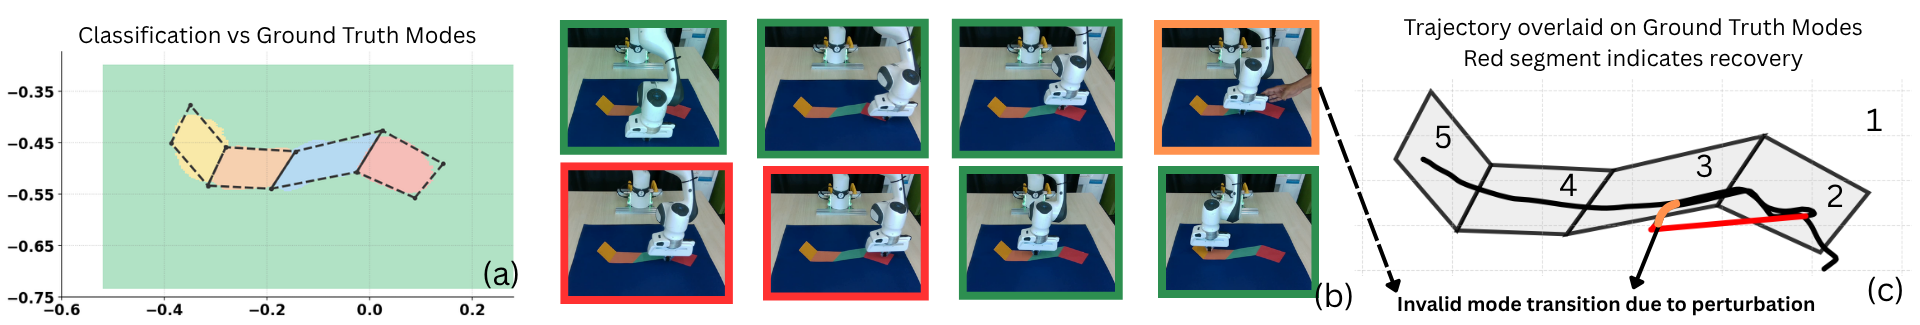
\includegraphics[width=\textwidth]{Figures/2d_nav_figure.png}
    \caption{\textbf{2D Navigation:} (a) the learned GPC boundaries match the ground truth; (b) a perturbation (orange) and the robot recovering (red) by following the correct mode sequence.}
    \label{fig:2d_recovery}
\end{figure*}

\subsection{2D Navigation (Simulation and Hardware)}
\label{sec:2d_nav}
% TODO(fig-consistency): make Fig.~\ref{fig:2d_recovery}/\ref{fig:comparison} visually
% seamless with Fig.~\ref{fig:seal_ltl_comp}, so the reader recognizes the 2D task as
% the "literal" instance of the Fig.~1 story:
%   1. Same visual language: guard curves in the seal green (dark, thick), initial safe
%      demos as solid seal!70 curves, queried states as filled dot + outer circle,
%      queried sub-demos as dashed seal!70 curves; GLiDE comparisons in the glide
%      orange with red x for oracle-labeled failures.
%   2. Panel (a) caption should say "guards" (the Fig.~1 term), not just "boundaries",
%      and note that here feature space = the physical workspace, so the guards of
%      Fig.~1 are literally visible.
%   3. Show the perturbation/recovery episode with the same red arrow + "recovery"
%      label styling as the automaton in Fig.~1.
%   4. If the figure is regenerated (matplotlib), pull colors from the paper palette:
%      seal RGB(0,140,90), glide RGB(200,120,0), tli RGB(80,80,80).
Replicated from GLiDE, the task is to traverse colored 2D regions in a prescribed order (Fig.~\ref{fig:comparison}a); here $F_{\min}$ is simply the $(x,y)$ coordinate. We request 6 demonstrations from mode~1 to mode~4 from varied starts, train an initial classifier, select 6 uncertain points, request 6 sub-demonstrations through them, and retrain on the combined 12. As boundary accuracy matters more than labeling the entire space here, we use margin uncertainty. We compare against GLiDE seeded with the same 6 demonstrations and its simulated perturbations.

Fig.~\ref{fig:comparison} shows that SEAL after active querying (b) closely matches the ground truth (a), and clearly improves on the pre-query classifier (c), demonstrating the value of active learning. Table~\ref{tab:miou_results} reports mean Intersection-over-Union (mIoU) against ground truth: SEAL matches GLiDE with 1000 perturbations, while GLiDE degrades sharply as its perturbation budget shrinks. We emphasize the correct accounting of effort (Q1): GLiDE's perturbations are cheap in simulation but require an outcome oracle and resets, whereas SEAL's additional cost is 6 human sub-demonstrations and no oracle; the comparison is thus of \emph{human effort and safety}, not raw sample count. Crucially, SEAL never accesses ground-truth labels during training, unlike GLiDE's success oracle. We do not claim to surpass GLiDE, which solves the harder problem of learning from sparse success/failure feedback; we show we can match it with a little more human effort and none of the oracle, perturbation, or reset machinery. \todoexp{random-query baseline (TODO.md A2): rerun with the 6 query points drawn uniformly at random at equal budget, add row to Table~\ref{tab:miou_results}, to isolate the value of uncertainty-targeted selection from that of extra data} \todoexp{sequence-aware baseline (TODO.md A3): HMM/windowed localizer trained on the same demos, measure miss rate/latency on perturbation-induced mode changes, to empirically back the memoryless design argument}

\begin{figure}[htbp]
\centerline{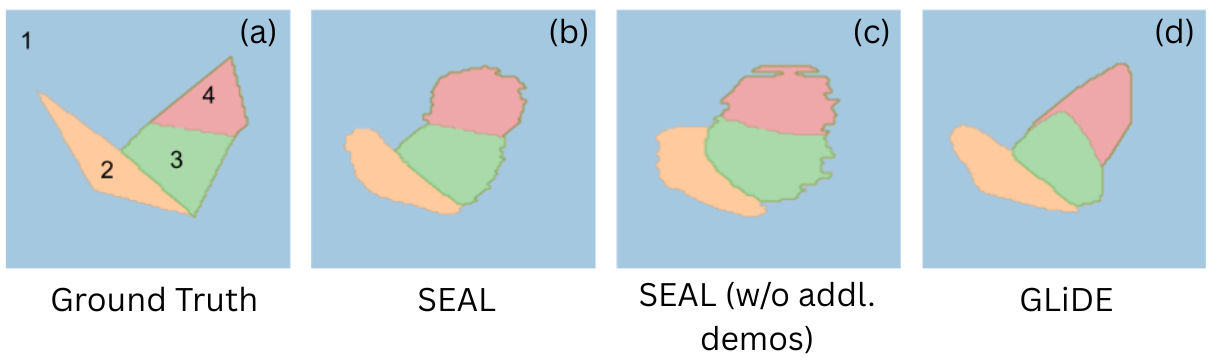
\includegraphics[width=0.5\textwidth]{Figures/comparison_GLiDE.png}}
\caption{Classification performance across methods. (a) ground-truth mode regions; (b) SEAL with 6+6 demonstrations; (c) SEAL without the active round (6 demonstrations); (d) GLiDE with 6 demonstrations + 1000 perturbed rollouts.}
\label{fig:comparison}
\end{figure}

\begin{table}[h]
    \centering
    \caption{Mean IoU Comparison on 2D Navigation}
    \label{tab:miou_results}
    \begin{tabular}{llc}
        \toprule
        \textbf{Method} & \textbf{Supervision} & \textbf{mIoU} \\
        \midrule
        SEAL (Ours) & 12 safe demos & \textbf{0.82} \\
        GLiDE & 6 demos + 1000 oracle rollouts & 0.80 \\
        SEAL (no active round) & 6 safe demos & 0.73 \\
        GLiDE & 6 demos + 400 oracle rollouts & 0.63 \\
        GLiDE & 6 demos + 100 oracle rollouts & 0.53 \\
        \bottomrule
    \end{tabular}
\end{table}

We replicate the task on a Franka FR3 7-DOF arm with 6+6 demonstrations; Fig.~\ref{fig:2d_recovery} shows the learned guards matching the ground-truth regions on hardware and a full perturbation--recovery episode, in which the localizer re-localizes the perturbed state and completes the prescribed sequence. \textbf{Empirical certificate (Q3).} We define the Level-1 certificate per rollout: an \emph{invariance violation} occurs if the feature trajectory exits $R_m$ through any boundary other than the nominal guard $G_{m,m'}$ (Definition~\ref{def:inv}), and \emph{reachability success} if it enters $G_{m,m'}$; rates are aggregated over unperturbed rollouts per mode. On this task we also evaluate the invariance/reachability-augmented acquisition of Sec.~\ref{sec:active}: \todo{report invariance-violation and reachability-success rates before vs.\ after guard-refinement queries}.

\subsection{Wiping}
This task evaluates reactive recovery in a continuous, contact-rich setting. A Franka FR3 with an eraser must clean a marker line across three modes---\textit{approach\_align}, \textit{wipe}, \textit{done}---and SEAL trains a supervisor from only 2 demonstrations. Random external forces break contact or displace the end-effector. The open-loop policy fails under perturbation, whereas the SEAL-supervised policy continues to the \textit{done} state, substantially improving the wiped fraction (Fig.~\ref{fig:robosuite_wiping}). Recovery emerges from localization: path displacement re-localizes \textit{wipe}$\to$\textit{approach\_align}, and incomplete cleaning re-localizes \textit{done}$\to$\textit{approach\_align}.

\begin{figure*}[t]
    \centering
    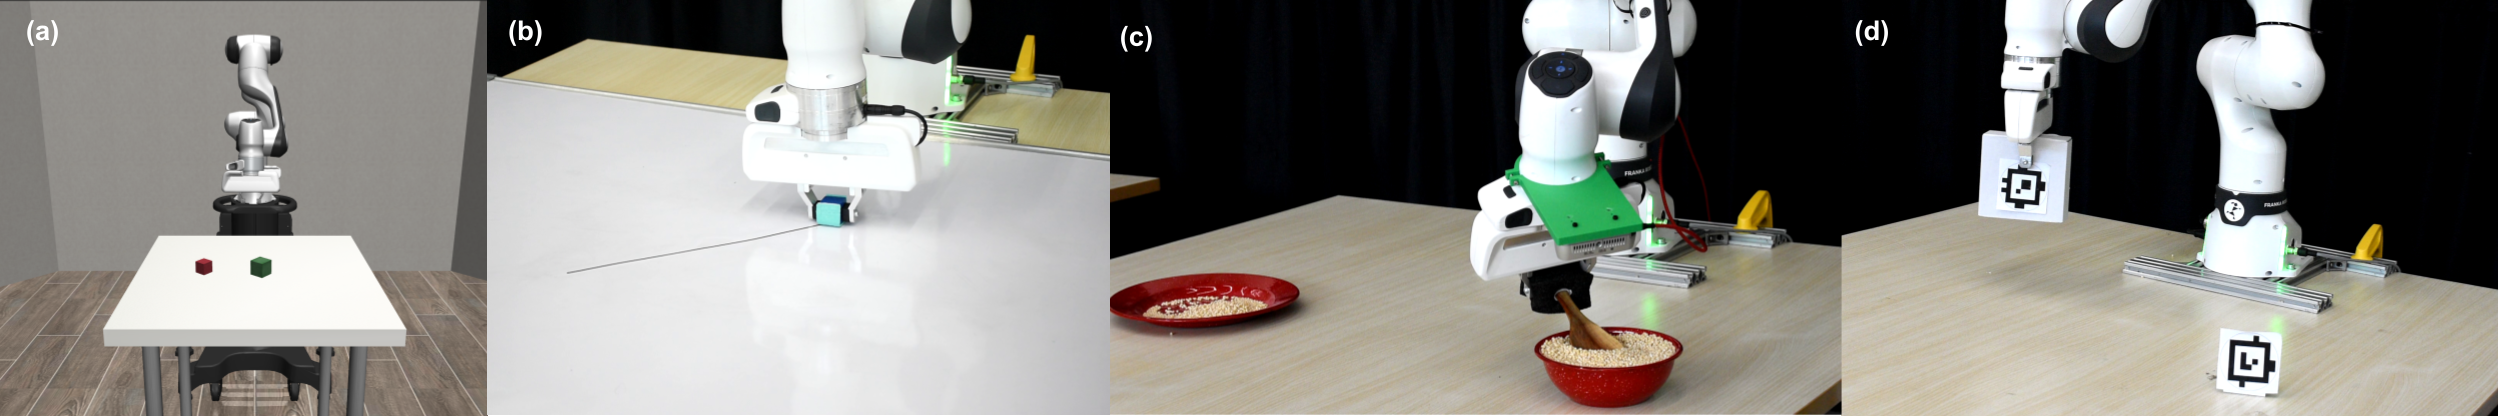
\includegraphics[width=\textwidth]{Figures/compilation.png}
    \caption{\textbf{Experimental setups:} Robosuite Stack (a), Wiping (b), Scooping (c), and Pick-and-Place (d).}
    \label{fig:compilation}
\end{figure*}

\begin{figure}[htbp]
\centerline{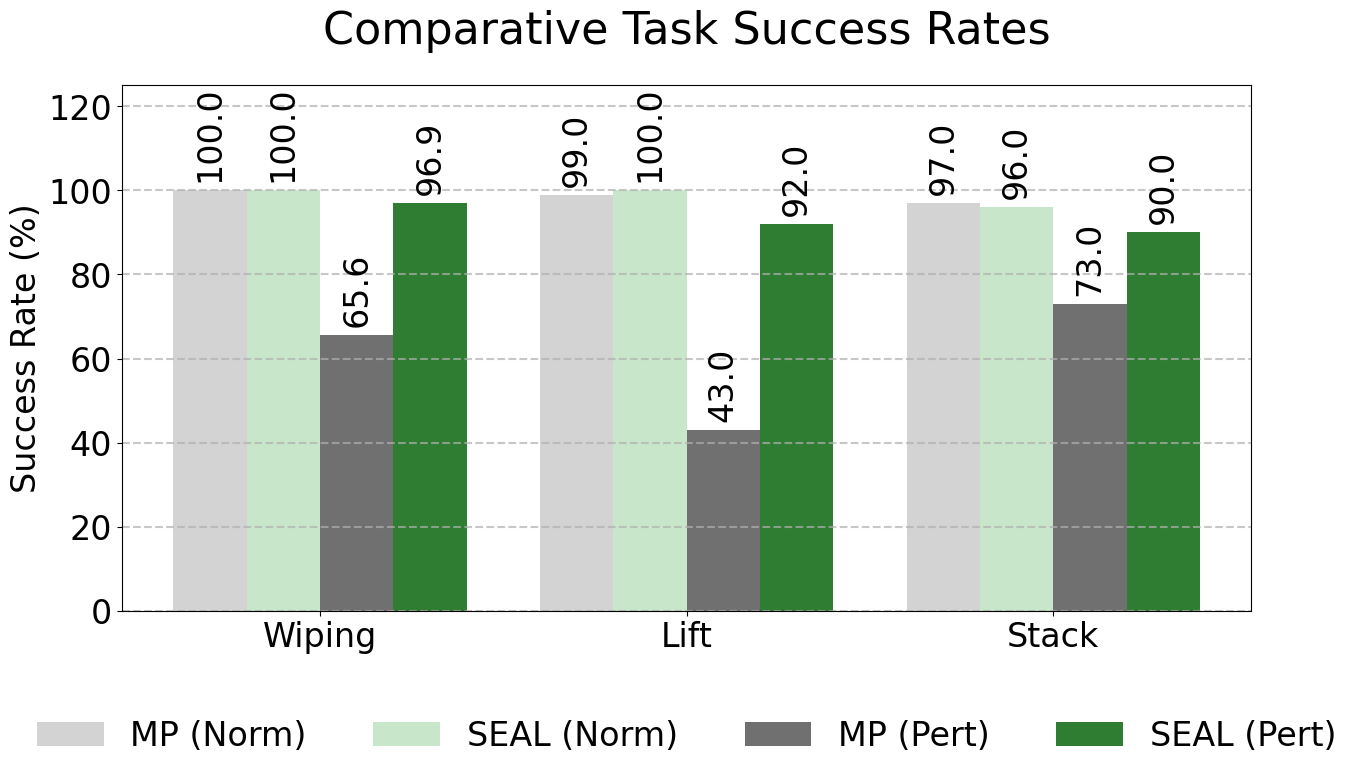
\includegraphics[width=0.5\textwidth]{Figures/robosuite_wiping.png}}
\caption{\textbf{SEAL supervision vs.\ open-loop policies on the Robosuite tasks (Wiping, Lift, Stack):} supervision causes no degradation without perturbations (light) and improves performance substantially under perturbations (dark).}
\label{fig:robosuite_wiping}
\end{figure}

\begin{figure*}[t]
    \centering
    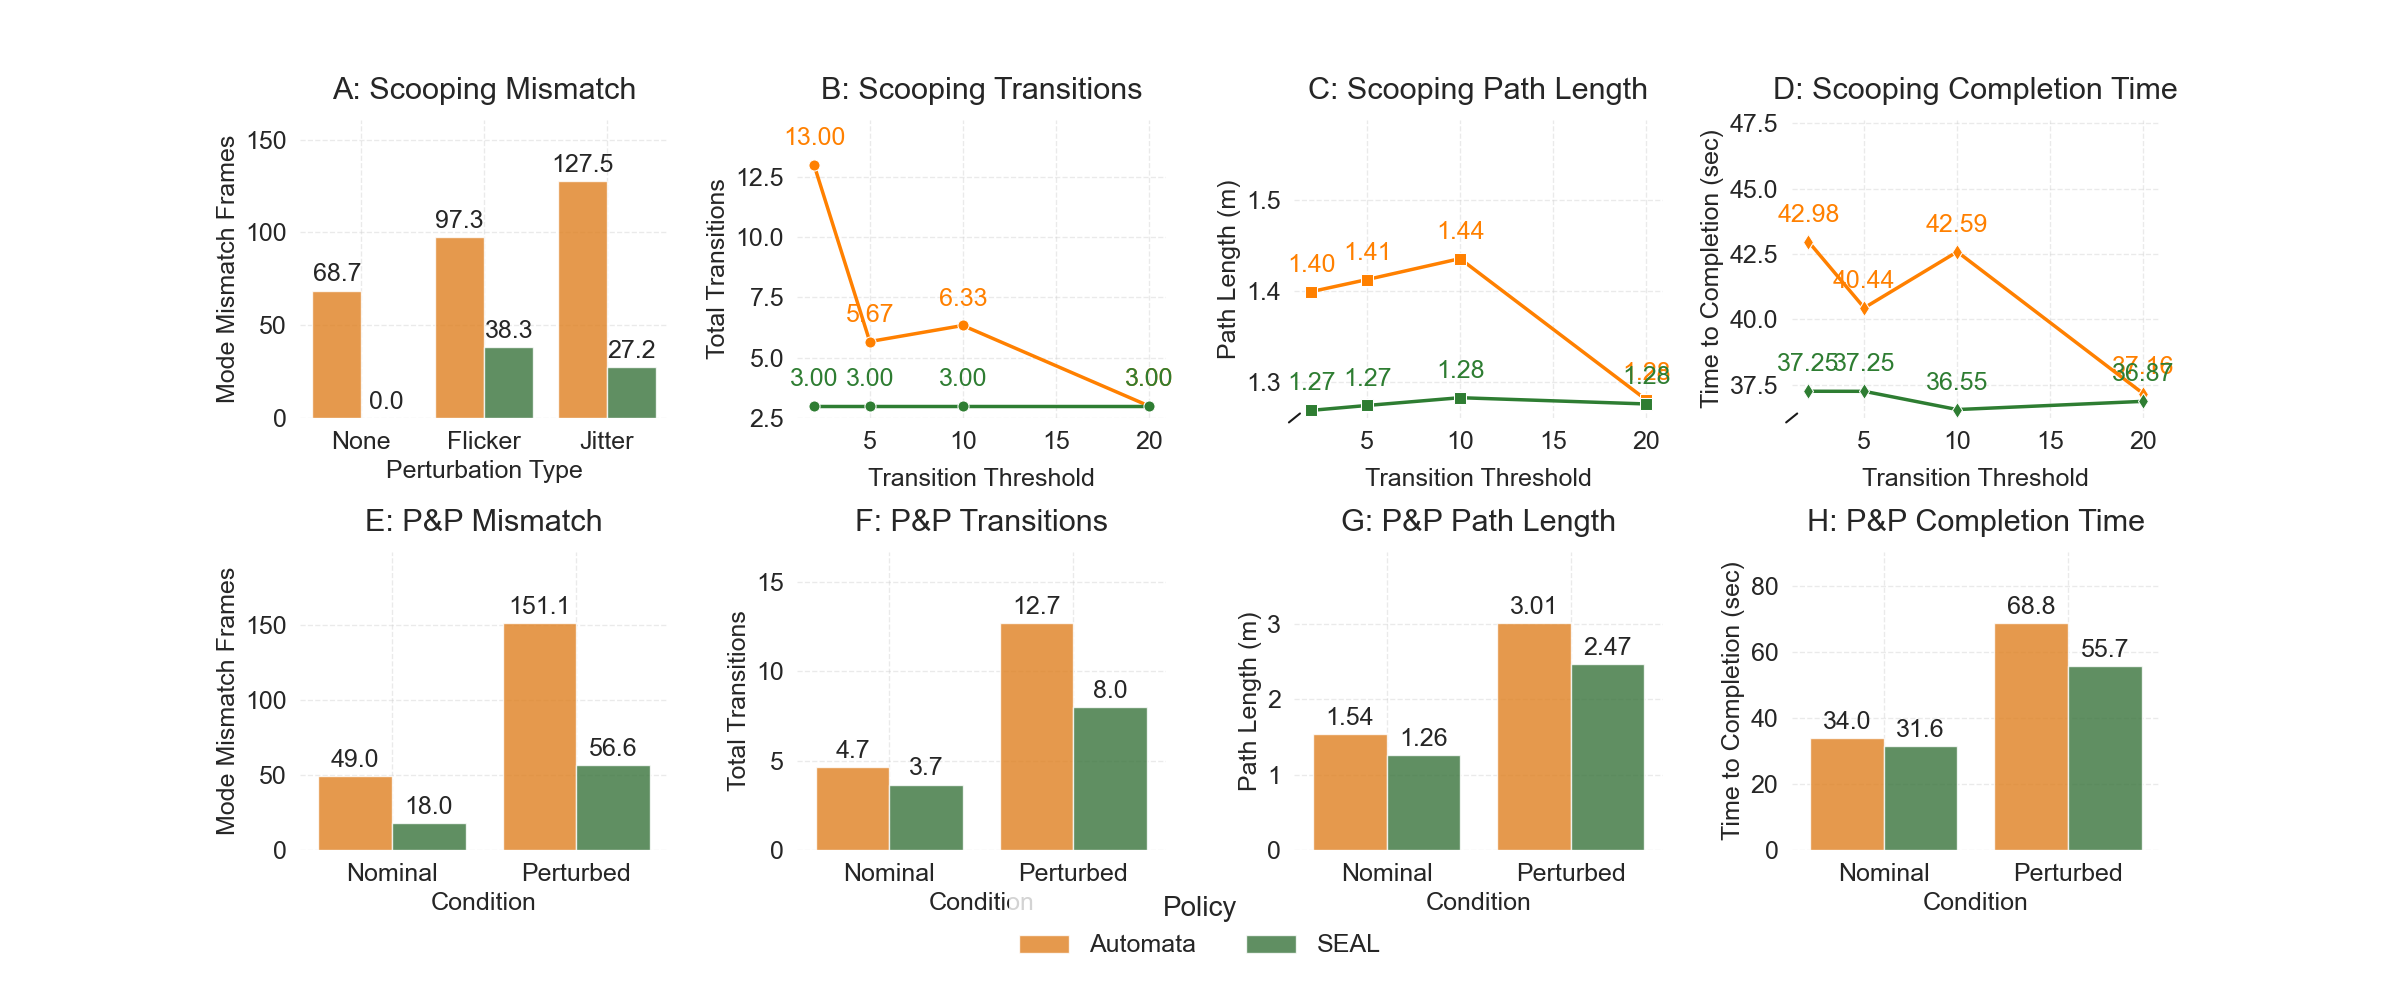
\includegraphics[width=\textwidth]{Figures/stacking_pnp.png}
    \caption{\textbf{Comparison with tuned automata.} In Scooping, confidence-gated transitions reduce false positives, yielding faster completion and shorter paths across thresholds. In Stacking, SEAL improves all efficiency metrics under both nominal and perturbed conditions. (Lower is better in all plots.)}
    \label{fig:scooping_pnp}
\end{figure*}

\subsection{Block Lifting and Stacking (Robosuite)}
We test non-monotonic features in the Lift and Stack environments~\cite{robosuite2020} (Fig.~\ref{fig:compilation}a). Gripper width is mapped to a binary \textit{grasped} feature to handle its non-monotonic profile, and relative end-effector-to-cube distances complete $F_{\min}$; SEAL trains on 7 demonstrations (3 nominal + 4 active) with separate continuous boundaries per gripper status---a case where the mixed-feature product kernel is useful. Over 100 episodes under random gripper perturbations, SEAL maintains a near-perfect nominal success rate and dramatically mitigates degradation under perturbation relative to open-loop (Fig.~\ref{fig:robosuite_wiping}).

\subsection{Scooping}
\label{sec:scooping}
We adopt GLiDE's scooping task: scoop, transport, and deposit rice from a bowl to a plate using a spoon on the end-effector. Open-loop execution fails at the task level if rice spills during transport or scooping fails---a case where failure demonstrations are hard to reset and self-supervised data collection is infeasible, so GLiDE cannot be run here. We detect grains on the spoon with a wrist camera (a binary feature) and use relative end-effector-to-bowl and -plate positions, training with 4 demonstrations.

Beyond comparison to open-loop, we ask how SEAL compares to a tuned automaton with expert-set thresholds---effectively an ideal, hand-built localizer that a learned classifier can only approximate but that is far harder to construct. We design and tune such an automaton on the same features. Because feature and prediction noise is unavoidable, especially near boundaries, \emph{all} classifiers---designed or learned---must confirm a switch over a small buffer to avoid false positives, trading latency against robustness. SEAL breaks this trade (Q2): with access to prediction confidence, it keeps a very small dwell and instead rejects low-confidence switches, smoothing boundary jitter; a genuine perturbation pushes the state deep into another region where confidence is high, giving a fast response. Thus SEAL attains low latency and low false-positive rate simultaneously. Note this reconciles the two roles of the automaton in our narrative: it is an accurate localizer, yet brittle to observation noise precisely because it lacks a calibrated confidence to gate on.

Over 24 trials spanning perturbation levels and transition thresholds (none inducing true task failure; these test observation-noise robustness), both policies achieve 100\% eventual completion---consistent with the learned localizer faithfully approximating the automaton; the per-mode certificate of Q3 (invariance-violation and reachability-success rates, as defined in Sec.~\ref{sec:2d_nav}) is reported separately: \todo{Level-1 certificate rates on scooping}. However, as the threshold shrinks, SEAL incurs no false-positive transitions while the automaton's rise (Fig.~\ref{fig:scooping_pnp}b), giving the automaton significantly higher completion times (d) and longer paths (c). As with any learned model, SEAL's accuracy depends on demonstration quality; a classifier trained on poor data cannot outperform a tuned automaton even with confidence gating. \todoexp{OOD-detector baseline (TODO.md A1): GMM--Mahalanobis detector (Eiband-style) trained on the same safe demos, evaluated on these perturbation episodes; report detection/false-positive rates next to SEAL's to substantiate the Related Work claim that time-conditioned OOD detectors do not transfer under spatial perturbation}

\subsection{Pick and Place}
The robot picks a box and places it near a target, both tracked with AprilTags~\cite{7759617} and a RealSense D435i. With gripper pick-and-place motions the base success rate is lower and failure demonstrations (object falling from the gripper) are potentially unsafe. We divide the task into \textit{Pick}, \textit{Transport}, \textit{Place}, and \textit{Retreat}, each with an object-conditioned primitive, and train from 2 demonstrations using relative distances and a binary gripper state. Over 42 trials with perturbations---moving objects during execution, inducing grasp failures and incorrect placements, and pulling the box from the gripper mid-transport---all efficiency metrics (completion time, path length) are again worse for the tuned automaton than for SEAL, though by a smaller margin than in scooping. Here we fix the transition threshold and instead vary start and goal positions to test generalization.

%%%%%%%%%%%%%%%%%%%%%%%%%%%%%%%%%%%%%%%%%%%%%%%%%%%%%%%%%%%%%%%%%%%%%%%%%%%%%%%%
\section{User Study: Restocking}
\label{sec:user_study}
All experiments so far used author-collected demonstrations. Because an LfD method's performance depends on the user, we conduct a study with 10 participants of varying familiarity with kinesthetic teaching and LfD, on a restocking task adapted from Ajanovi\'c et al.~\cite{11369949}. Their supermarket scenario used fixed object locations; our adaptation tracks the bottle and basket dynamically, so the localizer must generalize across spatial configurations. They found that users' preferences varied widely and that segmented demonstrations yielded slightly smoother, more successful policies at the cost of more demonstration time---supporting our use of segmented demonstrations.

\begin{figure*}[t]
    \centering
    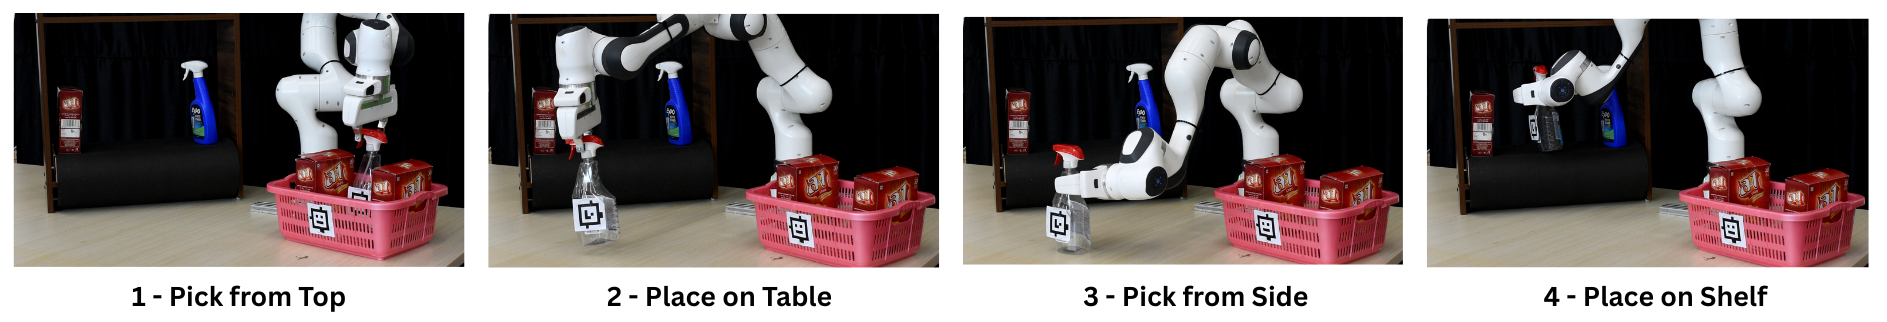
\includegraphics[width=\textwidth]{Figures/restocking_banner.png}
    \caption{\textbf{Restocking task.} The decomposition into \textit{Grasp\_Top}, \textit{Place\_Table}, \textit{Grasp\_Side}, \textit{Place\_Shelf} isolates the effect of SEAL's active-learning loop.}
    \label{fig:restocking_banner}
\end{figure*}

Because a cluttered basket forces a top grasp and a low shelf forces a side grasp, the task decomposes into \textit{Grasp\_Top}, \textit{Place\_Table}, \textit{Grasp\_Side}, \textit{Place\_Shelf} (Fig.~\ref{fig:restocking_banner}). We fix the features via the LLM so that only demonstration quality and diversity vary. The protocol: (1) participants give two segmented demonstrations aiming to maximize diversity (the \emph{Unguided} baseline); (2) we seed the GPC with the first demonstration and select 4 uncertain points (two gripper-open, two gripper-closed) via center-weighted epistemic uncertainty; (3) for each point we set up the corresponding scene and ask the participant to label and demonstrate the correct action to completion, yielding 4 sub-demonstrations that, with the first demonstration, form the \emph{SEAL Guided} set; (4) participants answer qualitative questions after each condition. We keep the count at 2 to probe the low-data regime and because participant frustration rose with more demonstrations; requesting 4 short sub-demonstrations (rather than 4 full ones) keeps the SEAL set comparable in points and collection time to the Unguided set while being more intuitive.

We test three hypotheses: (H1) even when asked to maximize diversity, users produce demonstrations with large state-space overlap; (H2) targeting uncertain, low-data regions yields a better classifier; (H3) users prefer the SEAL protocol. The final dataset comprises 20 sets (one Unguided, one SEAL per participant).

\textbf{Diversity (H1).} Since the first demonstration is shared, we measure the Mean Minimum Distance from points in subsequent demonstrations to same-mode points in the first,
\[
\text{MMD}(A,B)=\frac{1}{|B|}\sum_{b\in B}\min_{a\in A}\|a-b\|.
\]
The SEAL set ($\mu{=}0.247,\sigma{=}0.078$) is significantly more diverse than Unguided ($\mu{=}0.096,\sigma{=}0.108$), $t{=}4.17$ ($p<0.01$), confirming H1. Because classifier accuracy is a property of the data rather than of who staged the scene, this and the mIoU result below are robust to the scene-setup confound noted in Sec.~\ref{sec:limitations}.

\textbf{Classifier performance (H2).} We train 10 GPCs per dataset and report mIoU against a ground-truth classification defined by an independently hand-designed automaton over the full feature set (not from any trained model, hence non-circular). Focusing on the per-participant \emph{relative} change to control for individual expertise (Fig.~\ref{fig:participant_perf}), 7 of 10 participants improved with SEAL and 2 others changed within training-run variance, supporting H2. One participant (P09) declined markedly: they provided labels inconsistent with the ground-truth classification during the SEAL sub-demonstrations, underscoring the method's dependence on label quality (Sec.~\ref{sec:limitations}).

\begin{figure}[htbp]
\centerline{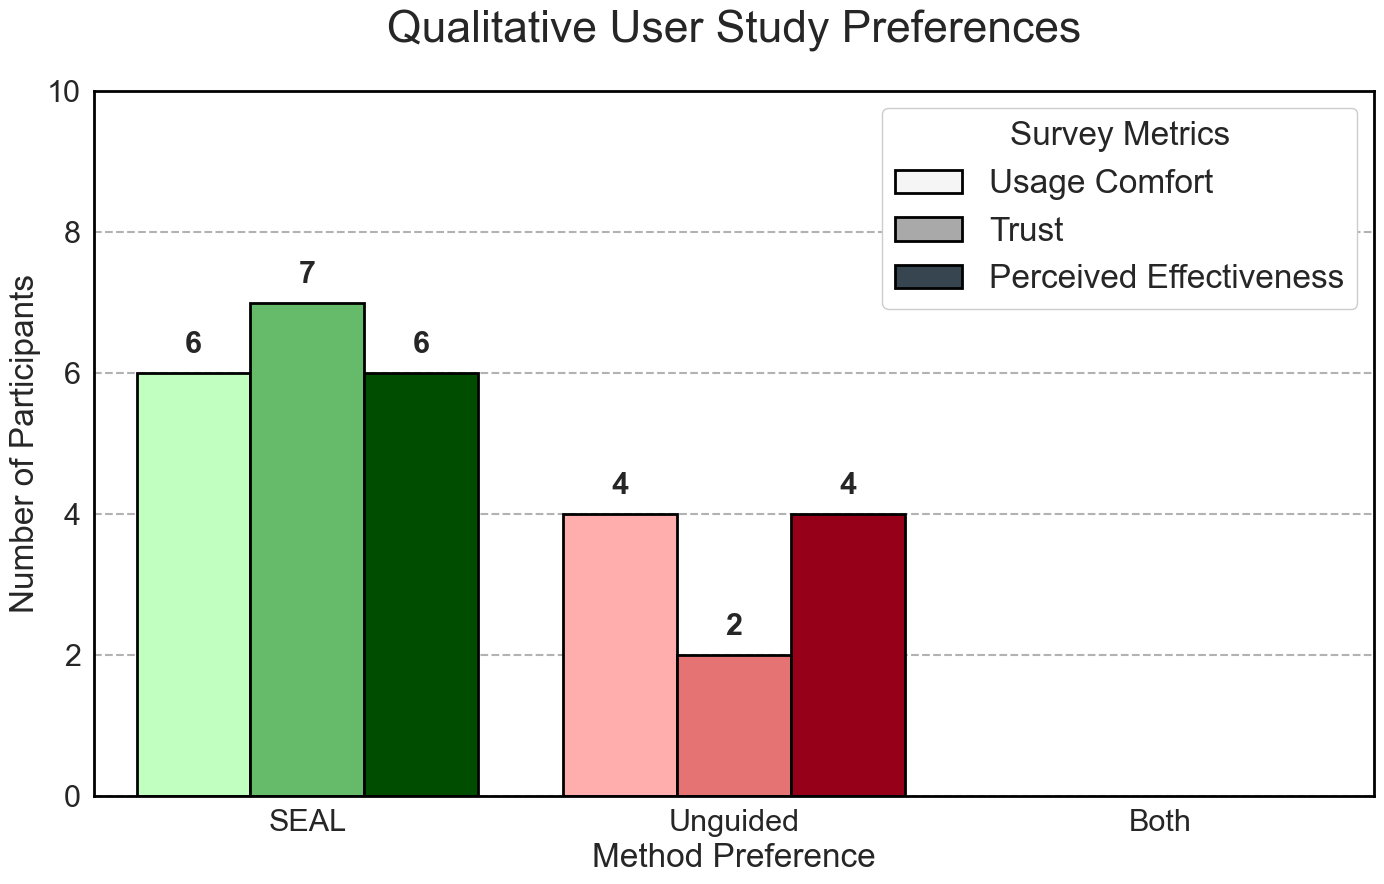
\includegraphics[width=0.5\textwidth]{Figures/pref.png}}
\caption{\textbf{User preferences:} more users prefer SEAL guidance over Unguided demonstrations on Comfort, Trust, and Perceived Effectiveness in a head-to-head comparison.}
\label{fig:user_pref}
\end{figure}

\begin{figure}[htbp]
\centerline{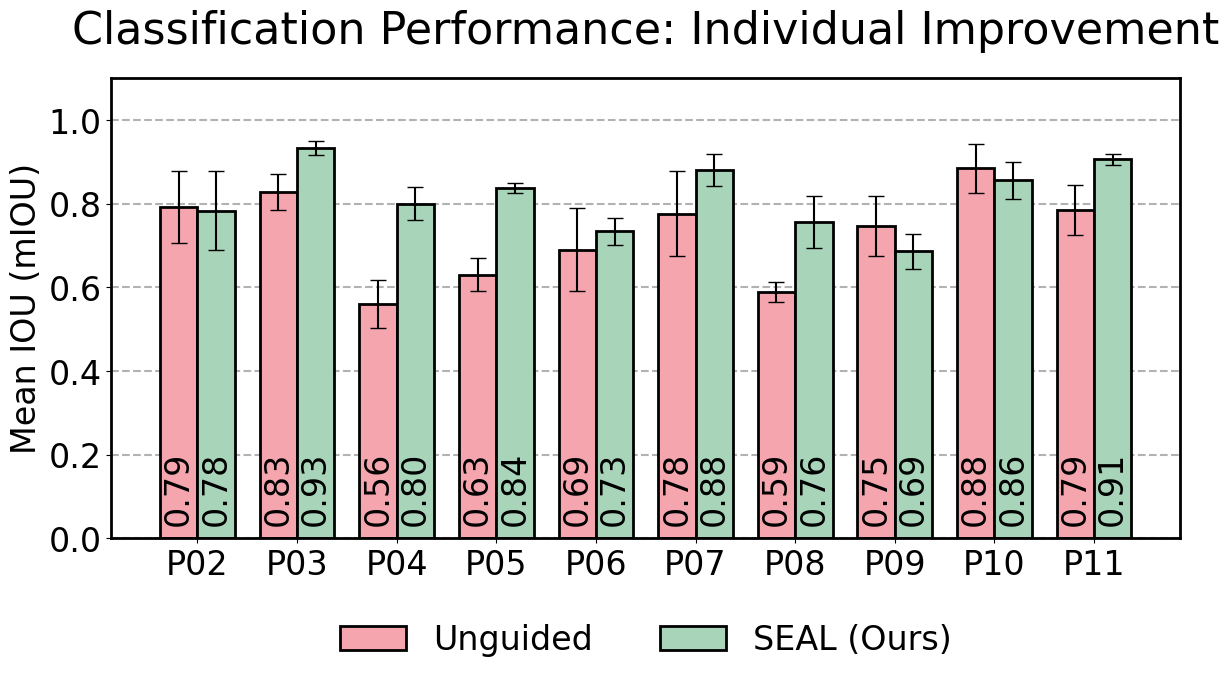
\includegraphics[width=0.5\textwidth]{Figures/miou.png}}
\caption{\textbf{mIoU per participant} for SEAL- and Unguided-trained models, averaged over 10 runs; error bars show $\pm1$ SD.}
\label{fig:participant_perf}
\end{figure}

\textbf{Preferences (H3).} More participants preferred SEAL on Ease of Use, Trust, and Efficiency (Fig.~\ref{fig:user_pref}). Self-reported mental effort dropped slightly with SEAL ($2.6\!\to\!1.8$, $p=0.125$), but physical-effort and ``how hard to achieve a good demonstration'' items showed no significant difference. H3 is thus only partially supported: SEAL is preferred head-to-head, but we cannot claim across-the-board preference at significance---consistent with our small sample and the confound below. Participants were similarly confident in both of their datasets, aligning with our intuition (H1) that users misjudge the diversity and downstream performance of their own demonstrations.

%%%%%%%%%%%%%%%%%%%%%%%%%%%%%%%%%%%%%%%%%%%%%%%%%%%%%%%%%%%%%%%%%%%%%%%%%%%%%%%%
\section{Conclusions and Limitations}
\label{sec:limitations}
We presented SEAL, which learns the localization function of a designed task automaton from a few safe demonstrations, letting multi-step LfD policies recover from task-level perturbations without hand-engineered sensor models or unsafe failure data. By framing the problem as mode localization, SEAL inherits goal reachability from goal-directed primitives and repurposes its calibrated classifier as a data-driven invariance monitor, matching expert-tuned automata and perturbation-based grounding at a fraction of the human and safety cost.

\textbf{Limitations.} (i) High-dimensional observations (images) cannot enter the active loop directly and must be processed into low-dimensional features; recent VLM-based segmentation of human videos~\cite{wang2024vlmseerobotdo} could relax this and enable learning from pre-existing demonstrations. (ii) In the user study, participants could not stage query scenes themselves and needed to see them physically before labeling, so the authors set up each scene---a genuine confound for the effort/preference measures (though not for diversity or mIoU) and a teaching bottleneck; visualizing query points for users is a clear next step. (iii) Performance depends on label quality (cf.\ P09); because we have runtime epistemic uncertainty, calibrating an uncertainty threshold to halt and re-query online is a direct remedy. (iv) We currently assume fixed primitives: if the environment changes so that a subtask always fails, SEAL cannot repair the primitive. The natural extension is to co-train the GPC with imitation-learned policies, which would let us \emph{establish}---rather than assume---mode invariance, and, since active queries target low-density regions, is expected to yield primitives with greater out-of-distribution robustness.

\appendices
\section{Classifier Architecture and Calibration}
\label{app:ablation}
\begin{figure*}[t]
\centering
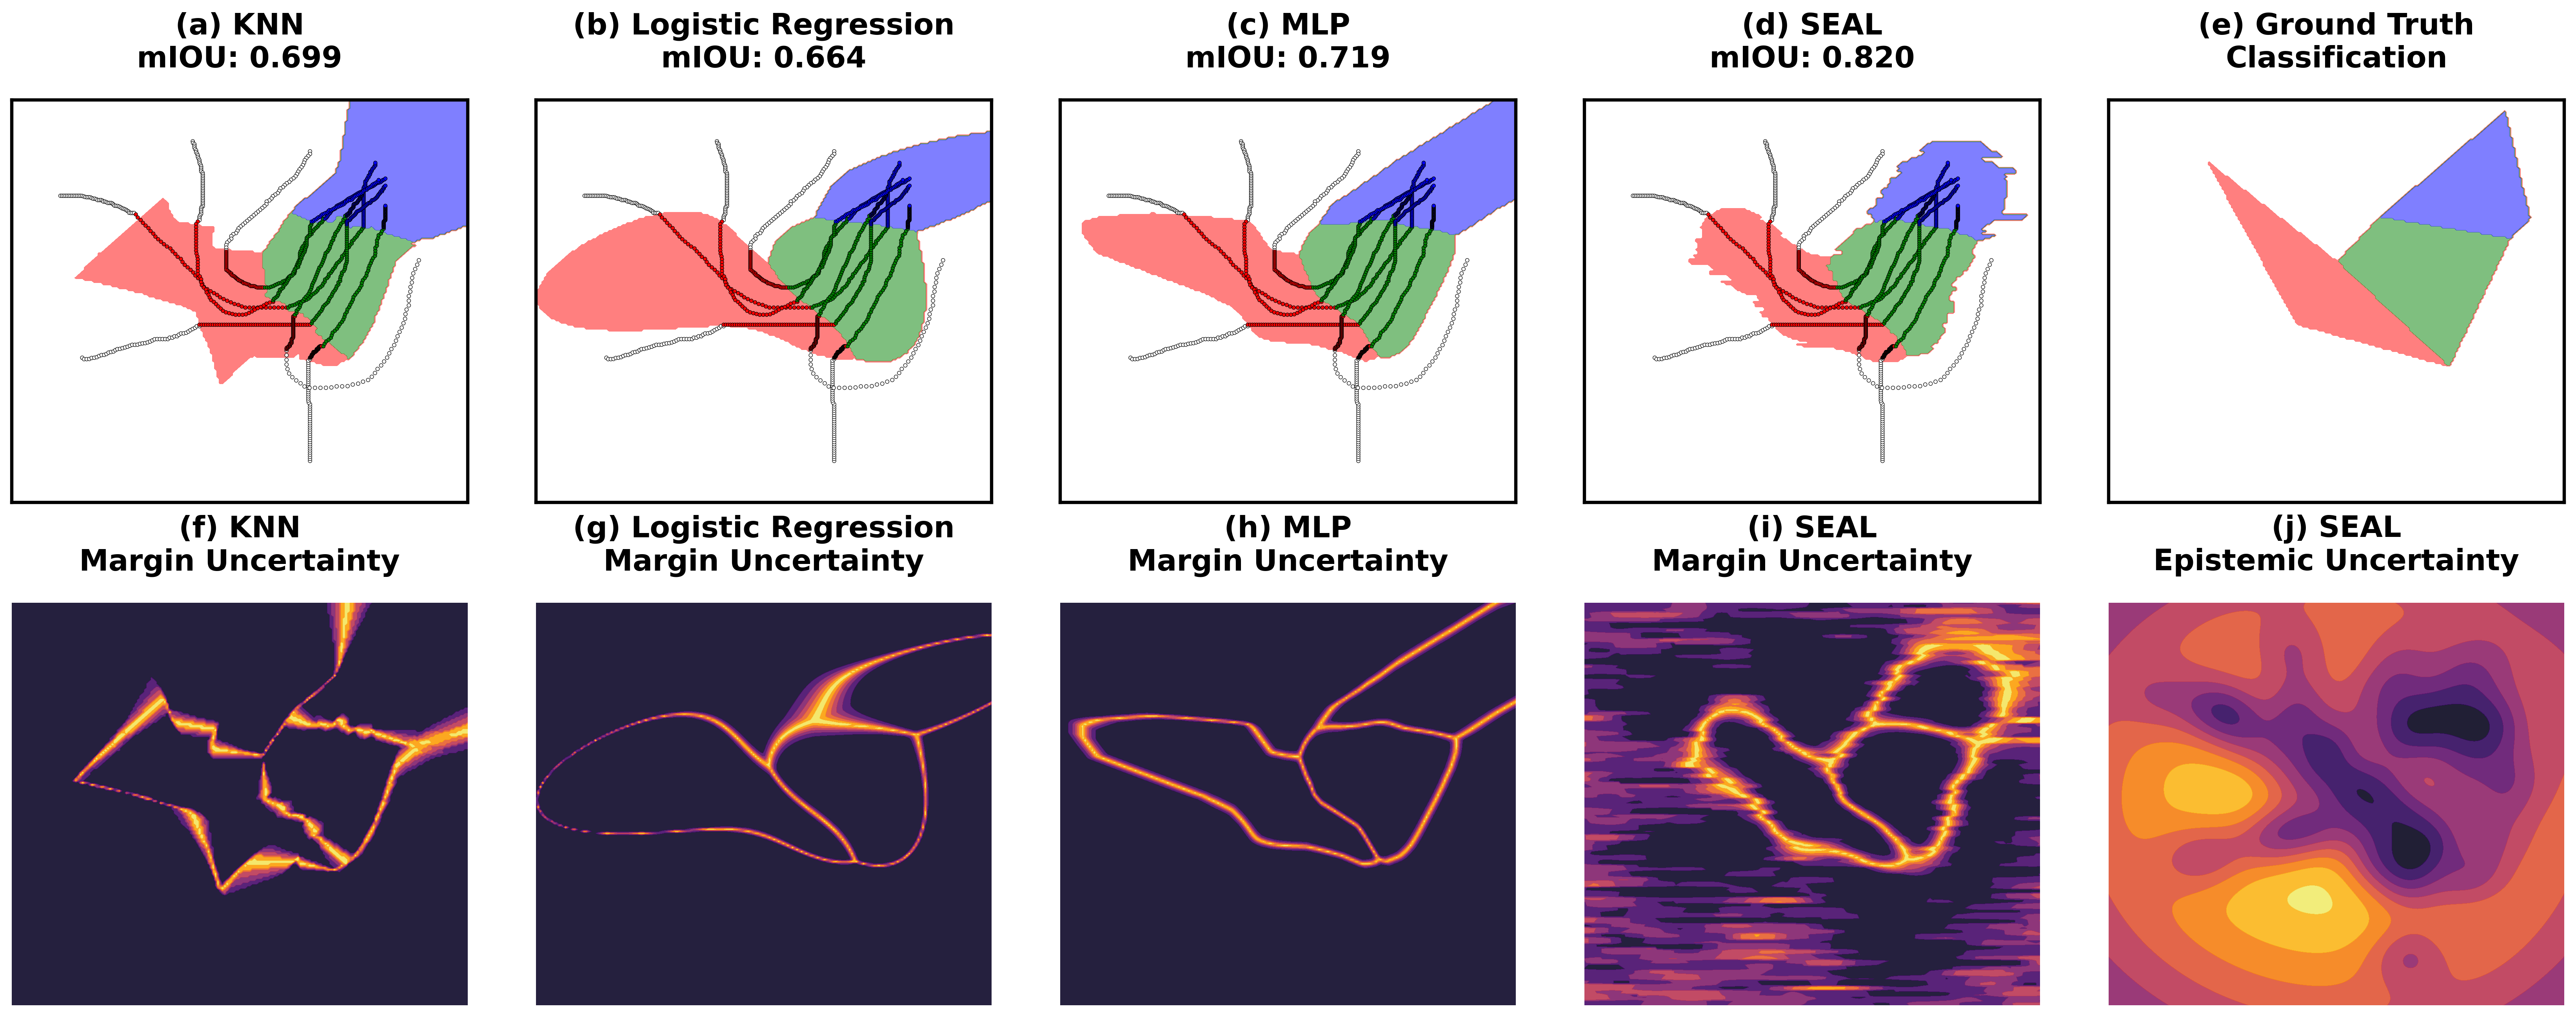
\includegraphics[width=1\textwidth]{Figures/ablation.png}
\caption{Performance of different classifier models; mIoU in brackets.}
\label{fig:ablation}
\end{figure*}
We ablate the classifier on the simulated 2D Navigation task, replacing the GPC with an MLP, logistic regression, and $k$-NN, all trained on the same data with hyperparameter tuning (Fig.~\ref{fig:ablation}). The simpler $k$-NN and logistic models underfit, while the MLP approaches the GPC's mIoU. However, unlike an MLP---which is overconfident far from training data---the GPC's posterior uncertainty grows where samples are sparse (Fig.~\ref{fig:ablation}f--j): the top-right region, unobserved in the initial demonstrations, is correctly flagged as uncertain by the GPC (i) while the MLP (h) stays confident. The GPC yields epistemic uncertainty (j) directly, without the expensive ensembling or MC-dropout other models require, and this drives active queries into informative, unexplored regions, making learning robust to sub-optimal initial demonstrations. \textbf{Calibration.} Because our confidence gating relies on the variational posterior, which can under-estimate uncertainty, we report a reliability diagram of the gated confidences and the resulting choice of $\tau$: \todo{insert calibration/reliability diagram and chosen $\tau$}. \textbf{Product kernel vs.\ independent GPs.} On the Stack task we compare the product kernel against fitting an independent GP per gripper state: \todo{report mIoU parity on binary contexts and the scaling advantage for $>2$ contexts}.

\section{Feature Selection: A Worked Example}
\label{app:feature}
The prompt supplied to the LLM in Stage~1 (Fig.~\ref{fig:framework}a) consists of a task-specific part and a fixed template:
\begin{itemize}
\item \textbf{Task-specific:} the task description (e.g., ``this is a pick and place task\,\dots''), the available raw features ($F_{\text{raw}}$, e.g., \texttt{EE\_pos}, \texttt{EE\_orn}, \texttt{Bottle\_pos}, \dots), and the target modes (e.g., \textit{Pick}, \textit{Transport}, \textit{Place}).
\item \textbf{Fixed template:} the LLM is instructed to act as a robotics engineer, to think \emph{prescriptively rather than descriptively}, to account for failures and perturbations, and to return a minimal list of processed features favoring spatially invariant relative quantities over absolute coordinates.
\end{itemize}
We argue that MI alone is insufficient for feature reduction: in the few-shot regime it cannot separate causal geometry from spurious spatial correlation. For instance, in restocking, replacing the relative end-effector-to-bottle angle with the \emph{absolute} angle yielded nearly identical MI, so MI cannot filter spatially dependent features---hence the LLM's invariance prior is required before mathematical verification. The following illustrates the end-to-end pipeline, showing how the MI certificate rejects an under-specified prompt and how ablation prunes the corrected set.

\textbf{Phase 1 (initial, under-specified prompt).} The operator omits that the bottle starts inside the basket:
\begin{quote}\small\itshape ``The objective is to restock the bottle onto the shelf. The robot must first establish a top grasp to lift the carton, place it on the table, transition to a side grasp, and finally place it on the shelf.''\end{quote}
The LLM proposes \{\textit{is\_grasped}, \textit{relative\_alignment}, \textit{z\_dist\_table}, \textit{z\_dist\_shelf}\}, whose $X_{\text{sel}}$ yields a joint MI of only $1.1036$ nats---well below the raw baseline $I(X_{\text{raw}};Y)\approx1.2737$ nats. The verification layer rejects it and requests a more descriptive prompt.

\textbf{Phase 2 (corrected prompt).} The operator adds the physical bottleneck:
\begin{quote}\small\itshape ``\dots When the carton is inside the basket, the robot can only grasp it from the top. If the carton is grasped from the top, the robot must place it on the table and regrasp it from the side before placing it on the tight shelf.''\end{quote}
The LLM outputs a spatially invariant set: $d_{\text{basket}}$ (carton--basket distance), $is_{\text{held}}$ (gripper boolean), $\theta_{\text{rel}}$ (end-effector--carton angle), and $h_{\text{carton}}$ (absolute carton height). Notably $h_{\text{carton}}$ is an absolute coordinate that slips through the invariance prior---an intentional illustration that the LLM can still propose a suboptimal feature, which the following minimization catches. This set yields $1.2704$ nats, matching the baseline; the system accepts it and proceeds.

\textbf{Phase 3 (minimization).} Dropping each feature and recomputing MI:
\begin{center}
\resizebox{\columnwidth}{!}{%
\begin{tabular}{@{}llc@{}}
\toprule
\textbf{Feature Set} & \textbf{MI (nats)} & \textbf{Information Loss ($\Delta$)} \\ \midrule
Full 4D Set (Baseline) & 1.2704 & -- \\ \midrule
Drop $d_{\text{basket}}$   & 1.1036 & $-0.1668$ (Critical) \\
Drop $is_{\text{held}}$    & 1.1429 & $-0.1275$ (Critical) \\
Drop $\theta_{\text{rel}}$ & 1.2399 & $-0.0305$ (Critical) \\
Drop $h_{\text{carton}}$   & \textbf{1.2706} & $\mathbf{+0.0002}$ (Redundant) \\ \bottomrule
\end{tabular}%
}
\end{center}
Omitting the absolute coordinate $h_{\text{carton}}$ incurs zero information loss, so it is discarded, finalizing the causally robust 3D space $F_{\min}=[d_{\text{basket}},is_{\text{held}},\theta_{\text{rel}}]$.

\bibliographystyle{/Users/ravi-imac/Library/CloudStorage/OneDrive-IndianInstituteofScience/Overleaf/SEAL/bib/IEEEtran}
\bibliography{/Users/ravi-imac/Library/CloudStorage/OneDrive-IndianInstituteofScience/Overleaf/SEAL/bib/example}
\end{document}
